% !TeX program = pdflatex
% !TeX encoding = UTF-8
\documentclass[aspectratio=169,compress,11pt]{beamer}

\usepackage[english]{babel}

\usepackage{Custom}
\usepackage{Custom-2}
\usepackage{AuxiliaryFiles/AuxiliaryFiles}
\usepackage{tabularx}

% Presenter notes mode.
% Use \presenternotesfalse when exporting the audience-only slide deck.
\newif\ifpresenternotes
\presenternotestrue
% \presenternotesfalse

\ifpresenternotes
  \setbeameroption{show notes on second screen=right}
\else
  \setbeameroption{hide notes}
\fi

% Thesis figures are kept in the thesis source tree so that the slides always
% use the same validated assets as the complete thesis.
\graphicspath{{../thesis_nsysu/Images/}}

% Presentation accents and reusable slide helpers.
\definecolor{Teal}{RGB}{0,132,137}
\definecolor{Gold}{RGB}{224,153,0}
\definecolor{SoftBlue}{RGB}{235,244,251}
\definecolor{SoftTeal}{RGB}{232,247,246}
\definecolor{SoftGold}{RGB}{255,247,224}
\setbeamercolor{takeaway}{fg=black,bg=SoftBlue}
\setbeamercolor{method}{fg=black,bg=SoftTeal}
\setbeamercolor{caution}{fg=black,bg=SoftGold}
\setbeamertemplate{itemize item}{\color{Teal}$\blacktriangleright$}
\setbeamertemplate{itemize subitem}{\color{Teal}$\vcenter{\hbox{\tiny$\bullet$}}$}
\setbeamertemplate{bibliography item}[text]

\newcommand{\ImageRoot}{../thesis_nsysu/Images}
\newcommand{\SlideCaption}[1]{%
  \par\vspace{0.4ex}{\centering\fontsize{5.5}{6.5}\selectfont\color{gray!80}#1\par}}
% Use the number assigned in the thesis rather than Beamer's local figure
% counter, because the presentation intentionally omits several thesis figures.
\newcommand{\ThesisFigureCaption}[2]{%
  \SlideCaption{\textbf{Figure #1.} #2}}
\newcommand{\SourceNote}[1]{%
  \par\vfill\hfill{\fontsize{5.3}{6.2}\selectfont\color{gray!80}#1}}
\newcommand{\Takeaway}[1]{%
  \begin{beamercolorbox}[rounded=true,sep=0.65ex,wd=\linewidth]{takeaway}
    \footnotesize\textbf{Takeaway:} #1
  \end{beamercolorbox}}
\newcommand{\MethodNote}[1]{%
  \begin{beamercolorbox}[rounded=true,sep=0.65ex,wd=\linewidth]{method}
    \footnotesize #1
  \end{beamercolorbox}}
\newcommand{\CautionNote}[1]{%
  \begin{beamercolorbox}[rounded=true,sep=0.65ex,wd=\linewidth]{caution}
    \footnotesize #1
  \end{beamercolorbox}}
\newcommand{\HC}[2]{\colorbox{#1}{\makebox[0.73cm][c]{\strut #2}}}

\begin{document}

\TitlePage
\SectionPage
\ProgressBar
\PageNumbering

\begin{frame}{Presentation Roadmap}
  \tableofcontents[hideallsubsections]

  \note{
    \begin{itemize}
      \item Narrative: physical focusing $\rightarrow$ validated channel effect
            $\rightarrow$ mobile system performance $\rightarrow$ the conditions
            under which angular selectivity becomes a communication benefit.
      \item Start from the physical focusing mechanism.
      \item Then connect the validated channel effect to mobile-system performance.
      \item Emphasize that angular selectivity is beneficial only under the
            conditions identified in this thesis.
    \end{itemize}
  }
\end{frame}

% !TEX root = ../BeamerTemplate.tex
%%%%%%%%%%%%%%%%%%%%%%%%%%%%%%%%%%%%%%%%%%%%%%%%%%%%%%%%%%%%%%%%%%%%%%%%%%%%%%%%%%

\section{Introduction}

\subsection{Research Context}

\begin{frame}[t]{Why 38~GHz? A High-Capacity Opportunity with a Spatial Cost}
\begin{columns}[T,onlytextwidth]
  \column{0.54\textwidth}
  \scriptsize
  \begin{itemize}
    \setlength{\itemsep}{-0.15em}
    \item Traffic growth and fragmented bands motivate mmWave \cite{Rappaport2013}.
    \item \textbf{38~GHz} is in FR2-1 / NR n260 (37--40~GHz), offering almost
          3~GHz of spectrum \cite{TSGR2021}.
    \item Short wavelengths enable compact arrays but intensify path loss,
          blockage, and sparse scattering \cite{Rappaport2013}.
    \item Directional gain is necessary; \emph{independent} channels remain
          difficult \cite{Payami2020}.
  \end{itemize}

  \column{0.42\textwidth}
  \centering
  \resizebox{\linewidth}{!}{%
  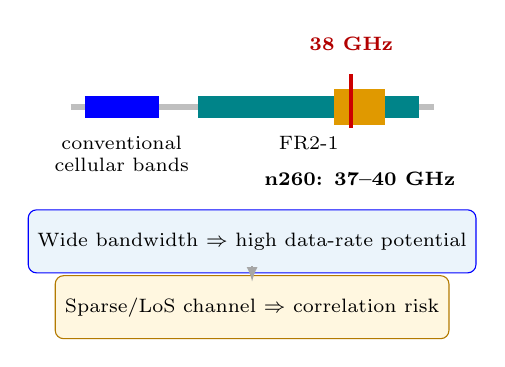
\begin{tikzpicture}[x=0.72cm,y=0.76cm,font=\scriptsize]
    \draw[gray!50,line width=2.2pt] (0,0)--(6.4,0);
    \draw[Blue,line width=8pt] (0.25,0)--(1.55,0);
    \node[below=7pt,align=center] at (0.9,0) {conventional\\cellular bands};
    \draw[Teal,line width=8pt] (2.25,0)--(6.15,0);
    \node[below=7pt] at (4.2,0) {FR2-1};
    \draw[Gold,line width=13pt] (4.65,0)--(5.55,0);
    \draw[red!80!black,line width=1.4pt] (4.95,-0.35)--(4.95,0.55);
    \node[above=5pt,text=red!70!black,font=\bfseries\scriptsize] at (4.95,0.55) {38~GHz};
    \node[below=20pt,font=\bfseries\scriptsize] at (5.1,0) {n260: 37--40~GHz};

    \node[draw=Blue,rounded corners=3pt,fill=SoftBlue,
          minimum width=5.0cm,minimum height=0.8cm,align=center] at (3.2,-2.25)
          {Wide bandwidth $\Rightarrow$ high data-rate potential};
    \node[draw=Gold!80!black,rounded corners=3pt,fill=SoftGold,
          minimum width=5.0cm,minimum height=0.8cm,align=center] at (3.2,-3.35)
          {Sparse/LoS channel $\Rightarrow$ correlation risk};
    \draw[-latex,thick,gray!70] (3.2,-2.67)--(3.2,-2.92);
  \end{tikzpicture}}
\end{columns}

\note{
    \begin{itemize}
      \item Conventional cellular bands are crowded; so we move to mmWave Band is a solution.
      \item Which mean 38~GHz is a good candidate for high data rate, but the channel is sparse and LoS dominant.
      \item The bandwidth is wide on FR2-1 especially n260 offer 3ghz of spectrum, high data rate potential, but the channel is sparse and LoS dominant.
      \item Spatial multiplexing depends on $\mathbf H$, not bandwidth or antenna count.
    \end{itemize}
  }
\end{frame}


\begin{frame}[t]{The Conventional mmWave MIMO Dilemma}
\small
\begin{columns}[T,onlytextwidth]
  \column{0.315\textwidth}
  \begin{block}{Fully digital}
    \centering\textbf{1 RF chain / element}\par
    \vspace{0.25cm}
    \raggedright
    \textcolor{green!60!black}{$+$ Maximum precoding flexibility}\par
    \textcolor{green!60!black}{$+$ Multiple streams}\par
    \textcolor{red!75!black}{$-$ Cost, power, calibration}
  \end{block}

  \column{0.315\textwidth}
  \begin{block}{Analog}
    \centering\textbf{1 RF chain / beam} \cite{Zeng2018}\par
    \vspace{0.25cm}
    \raggedright
    \textcolor{green!60!black}{$+$ High array gain}\par
    \textcolor{green!60!black}{$+$ Lower RF complexity}\par
    \textcolor{red!75!black}{$-$ Typically one data stream}
  \end{block}

  \column{0.315\textwidth}
  \begin{block}{Hybrid}
    \centering\textbf{Few RF chains} \cite{Payami2020}\par
    \vspace{0.25cm}
    \raggedright
    \textcolor{green!60!black}{$+$ Gain--multiplexing trade-off}\par
    \textcolor{red!75!black}{$-$ Phase shifters and RF routing}\par
    \textcolor{red!75!black}{$-$ Insertion loss / wideband design}
  \end{block}
\end{columns}

\note{
    \begin{itemize}
      \item There's 3 types of mmWave MIMO architecture, fully digital, analog, and hybrid. they have their own advantages and disadvantages.
      \item Fully digital has maximum precoding flexibility and multiple streams, but it is costly, power hungry, and calibration is difficult.
      \item Analog has high array gain and lower RF complexity, but it typically supports only one data stream.
      \item Hybrid offers a gain-multiplexing trade-off, but it has phase shifters and RF routing issues, as well as insertion loss and wideband design challenges.
      \item In a LoS-dominant channel, similarly oriented antennas can observe
            nearly the same field: $|\rho_{ij}|\!\rightarrow\!1$,
            $\sigma_3\!\rightarrow\!0$, and adding elements does \textbf{not}
            guarantee more usable spatial streams.
      \item so in this thesis, we will explore the metasurface lens as a passive spatial transformer to improve the MIMO channel beyond received-power gain.
    \end{itemize}
  }
\end{frame}


\subsection{Lens-Assisted Beamspace MIMO}

\begin{frame}[t]{Metasurface Lens as a Passive Spatial Transformer}
\scriptsize
\begin{columns}[T,onlytextwidth]
  \column{0.41\textwidth}
  \begin{itemize}
    \setlength{\itemsep}{0em}
    \item Sub-wavelength cells impose a position-dependent transmission phase
          \cite{Al-Joumayly2011}.
    \item By reciprocity, different arrival angles focus at distinct points
          \cite{Zeng2016}.
    \item The lens maps \textbf{antenna space} to \textbf{beamspace} in the
          electromagnetic domain \cite{Zeng2016}.
    \item No active phase shifter is required per aperture element
          \cite{Shen2019}.
  \end{itemize}

  \column{0.55\textwidth}
  \centering
  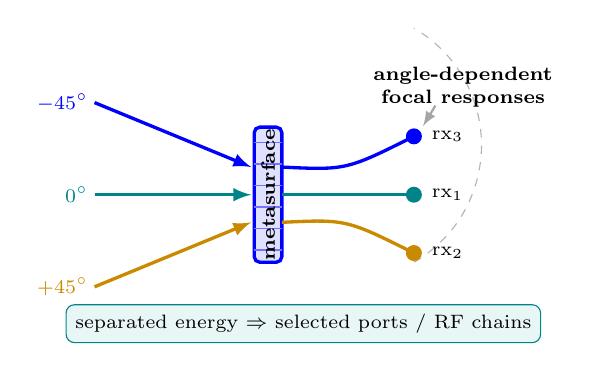
\begin{tikzpicture}[x=0.78cm,y=0.78cm,>=latex,font=\scriptsize]
    % Incident angular paths
    \draw[Blue,very thick,-latex] (-0.4,2.4)--(2.15,1.35);
    \draw[Teal,very thick,-latex] (-0.4,0.9)--(2.15,0.9);
    \draw[Gold!90!black,very thick,-latex] (-0.4,-0.6)--(2.15,0.45);
    \node[Blue,left] at (-0.35,2.4) {$-45^\circ$};
    \node[Teal,left] at (-0.35,0.9) {$0^\circ$};
    \node[Gold!90!black,left] at (-0.35,-0.6) {$+45^\circ$};
  
    % Metasurface aperture
    \draw[rounded corners=2pt,fill=Blue!12,draw=Blue,very thick]
      (2.2,-0.2) rectangle (2.65,2.0);
    \foreach \y in {0.0,0.35,...,1.85}{\draw[Blue!55] (2.2,\y)--(2.65,\y);}
    \node[rotate=90,font=\bfseries\scriptsize] at (2.425,0.9) {metasurface};
  
    % Focused paths
    \draw[Blue,very thick] (2.65,1.35)..controls(3.7,1.3)..(4.8,1.85);
    \draw[Teal,very thick] (2.65,0.9)..controls(3.7,0.9)..(4.8,0.9);
    \draw[Gold!90!black,very thick] (2.65,0.45)..controls(3.7,0.5)..(4.8,-0.05);
    \draw[gray!60,dashed] (4.8,-0.2) arc[start angle=-60,end angle=60,radius=2.2];
  
    \foreach \p/\c/\lab in {(4.8,1.85)/Blue/$\mathrm{rx}_3$,
                              (4.8,0.9)/Teal/$\mathrm{rx}_1$,
                              (4.8,-0.05)/Gold!90!black/$\mathrm{rx}_2$}{
      \fill[\c] \p circle (0.13);
      \node[right=3pt] at \p {\lab};
    }
    \node[align=center,font=\bfseries\scriptsize] at (5.6,2.65)
      {angle-dependent\\focal responses};
    \draw[-latex,thick,gray!70] (5.15,2.35)--(4.95,2.02);
  
    \node[draw=Teal,rounded corners=3pt,fill=SoftTeal,align=center,
          minimum width=5.2cm] at (3.0,-1.2)
      {separated energy $\Rightarrow$ selected ports / RF chains};
  \end{tikzpicture}
\end{columns}

\note{
    \begin{itemize}
      \item The metasurface lens is a passive spatial transformer that maps antenna space to beamspace.
      \item It uses sub-wavelength cells to impose a position-dependent transmission phase, which focuses different arrival angles at distinct points(focal arc).
      \item This allows for separated energy and selected ports or RF chains without the need for active phase shifters per aperture element. or simplify like Angle filter, but with lower cost, power, and complexity.
      \item Target: a direction-selective MIMO channel matrix $\mathbf H$, not
            aperture gain alone.
    \end{itemize}
  }
\end{frame}


\subsection{Literature Gap}

\begin{frame}[t]{What Prior Work Established --- and What Remains Open}
\scriptsize
\setlength{\tabcolsep}{3pt}
\renewcommand{\arraystretch}{1.12}
\newcommand{\grayrowrule}{%
  \noalign{\vskip 1pt\begingroup\color{gray!35}\hrule height 0.3pt\endgroup\vskip 1pt}}
\begin{tabularx}{\linewidth}{
  >{\raggedright\arraybackslash}p{2.05cm}
  >{\raggedright\arraybackslash}p{2.20cm}
  >{\raggedright\arraybackslash}X
  >{\raggedright\arraybackslash}X}
  \toprule
  \textbf{Representative work} & \textbf{Physical system} &
  \textbf{What it established} & \textbf{Limitation relevant here} \\
  \midrule
  Al-Joumayly \& Behdad \cite{Al-Joumayly2011} & X-band MEFSS lens &
  Wideband sub-wavelength spatial phase shifters &
  Multilayer, primarily antenna-level evaluation \\
  \grayrowrule
  Lee \textit{et al.} (2021) \cite{Lee2021} & 38~GHz, $13\!\times\!13$ lens &
  35--40~GHz focusing and incident-angle stability &
  Scalability to a substantially larger aperture not shown \\
  \grayrowrule
  Lee \textit{et al.} (2022) \cite{Lee2022Large} & 28~GHz, $28\!\times\!28$ lens &
  Large-aperture gain and throughput improvement &
  Limited channel-decorrelation and spatial-mode analysis \\
  \grayrowrule
  Zeng / Shen \textit{et al.} \cite{Zeng2016,Shen2019} & Analytical lens arrays &
  Beam selection, RF-chain reduction, path multiplexing &
  Idealized response; finite aperture and physical errors omitted \\
  \bottomrule
\end{tabularx}

\vspace{0.15cm}
\begin{columns}[T,onlytextwidth]
  \column{0.48\textwidth}
  \MethodNote{\textbf{Physical-lens studies:} phase, focus, gain, bandwidth.}
  \column{0.48\textwidth}
  \MethodNote{\textbf{Communication studies:} sparsity, selection, capacity.}
\end{columns}

\note{
    \fontsize{8.5}{9.5}\selectfont
    \begin{itemize}
      \setlength{\itemsep}{0.25em}
      \setlength{\parskip}{0pt}
      \item Al-Joumayly and Behdad's work focused on X-band MEFSS lens, which established wideband sub-wavelength spatial phase shifters, but it was primarily an antenna-level evaluation. His idea is most easy to understand, but it is not a complete system-level evaluation.
      \item Wonwoo Lee et al. (2021) worked on a 38~GHz, $13\times13$ lens, which demonstrated focusing and incident-angle stability, but scalability to a larger aperture was not shown. which is close to our work bandwidth.
      \item Korean Samsung Engineer(Jaehyun Lee) publish about MIMO Transmission for 6G Lee et al. (2022) worked on a 28~GHz, $28\times28$ lens, which improved large-aperture gain and throughput, but had limited channel-decorrelation and spatial-mode analysis. it is close to our work, but the frequency is different. and as last time i track his paper, this is his last published paper about antenna-lens.
      \item If i not worng In Singapore, Yong Zeng and Rui Shen et al. worked on analytical lens arrays, which focused on beam selection, RF-chain reduction, and path multiplexing, but their work was idealized and omitted finite aperture and physical errors. Yong Zeng's work Path Division Multiplexing influence our work, make me understand the concept of beamspace MIMO. Most of his published paper that i read usually use idealized lens response, and his published paper about antenna-lens MIMO in 2021, which is collaboration with Prof. Wen writing about Extreme Large Lens Antenna arrays. At this moment, i little bit nerveous because Prof. Wen become my oral defense committee member. 
      \item \textit{Optional to say:} The missing bridge is a physical
            metasurface response evaluated as a MIMO channel, not merely as an
            antenna-gain device.
    \end{itemize}
  }
\end{frame}


\begin{frame}[t]{Four Research Gaps Define the Thesis}
\footnotesize
\begin{itemize}
  \setlength{\itemsep}{0.25em}
  \item[\textbf{1.}] \textbf{Electromagnetics $\leftrightarrow$ communications:}
        Physical focusing and the resulting MIMO matrix have rarely been
        evaluated in one consistent workflow \cite{Lee2022Large,Bagheri2023}.
  \item[\textbf{2.}] \textbf{38~GHz aperture scalability:}
        Prior 38~GHz work did not establish substantially larger-aperture
        performance \cite{Lee2021}.
  \item[\textbf{3.}] \textbf{Practical focal-plane placement:}
        Finite spot width, sidelobes, loss, phase error, and diffraction can
        make neighboring focal responses overlap.
  \item[\textbf{4.}] \textbf{Controlled array comparison:}
        Lens-assisted focal-plane and conventional coplanar arrays must be
        compared under matched geometry, power, bandwidth, and noise
        assumptions.
\end{itemize}

\vspace{-0.15cm}
\CautionNote{\centering\textbf{Antenna-gain enhancement alone does not establish
an improvement in spatial multiplexing.}}
\note{
    \fontsize{7}{8}\selectfont
    \begin{itemize}
      \setlength{\itemsep}{0.3em}
      \setlength{\parskip}{0pt}
      \item This slide summarizes the four gaps that motivate my thesis.
      \item First, electromagnetic studies usually report phase, focusing, and
            antenna gain, while communication studies analyze the channel
            matrix. These two perspectives are rarely evaluated together in
            one consistent workflow.
      \item Second, earlier work close to 38~GHz demonstrated a $13\!\times\!13$
            lens. My work investigates a larger $20\!\times\!20$ aperture and
            checks whether its designed phase response still produces the
            intended focusing behavior.
      \item Third, a practical focus is not an ideal point. Finite spot width,
            sidelobes, loss, phase error, and diffraction can cause adjacent
            focal responses to overlap, so antenna placement along the focal
            region must be evaluated carefully.
      \item Fourth, a fair lens-versus-baseline comparison requires consistent
            operating assumptions, including frequency, bandwidth, transmit
            power, noise, propagation environment, and array order.
      \item The key message is that higher antenna gain only proves stronger
            received power. A spatial-multiplexing improvement must also be
            supported by the channel correlation, singular values, effective
            rank, and MIMO capacity.
    \end{itemize}
  }
\end{frame}


\subsection{Research Question and Objectives}

\begin{frame}[t]{Research Logic and Testable Component-Level Hypothesis}
\begin{beamercolorbox}[rounded=true,sep=1.0ex,wd=\linewidth]{takeaway}
  \centering\large\bfseries
  Can a physical 38~GHz transmitarray create distinct angle-dependent responses
  that alter the MIMO channel beyond received-power gain?
\end{beamercolorbox}

\vspace{0.55cm}
\centering
\begin{tikzpicture}[node distance=0.55cm,>=latex,font=\scriptsize]
  \node[draw=Blue,fill=SoftBlue,rounded corners,minimum width=2.55cm,
        minimum height=0.85cm,align=center] (focus) {physical lens\\focusing};
  \node[draw=Teal,fill=SoftTeal,rounded corners,minimum width=2.55cm,
        minimum height=0.85cm,align=center,right=of focus] (matrix) {less overlap in\\$\mathbf H$};
  \node[draw=Gold!80!black,fill=SoftGold,rounded corners,minimum width=2.55cm,
        minimum height=0.85cm,align=center,right=of matrix] (modes) {more balanced\\$\sigma_1,\sigma_2,\sigma_3$};
  \node[draw=Blue,fill=SoftBlue,rounded corners,minimum width=2.55cm,
        minimum height=0.85cm,align=center,right=of modes] (perf) {better MIMO\\performance};
  \draw[->,thick] (focus)--(matrix);
  \draw[->,thick] (matrix)--(modes);
  \draw[->,thick] (modes)--(perf);
\end{tikzpicture}

\vspace{0.6cm}
\begin{columns}[T,onlytextwidth]
  \column{0.19\textwidth}\centering
    $|\rho_{ij}|\,\downarrow$\\[-1pt]{\scriptsize decorrelation}
  \column{0.19\textwidth}\centering
    $\kappa\,\downarrow$\\[-1pt]{\scriptsize better conditioning}
  \column{0.19\textwidth}\centering
    $r_{\mathrm{eff}}\,\uparrow$\\[-1pt]{\scriptsize more modes}
  \column{0.19\textwidth}\centering
    $C_{\mathrm{raw}}\,\uparrow$\\[-1pt]{\scriptsize link-budget benefit}
  \column{0.19\textwidth}\centering
    $|H_{ii}|/|H_{ij}|\,\uparrow$\\[-1pt]{\scriptsize angular selectivity}
\end{columns}

\SourceNote{Chapter 1: Motivation and Research Gaps}
\note{
  \fontsize{7}{8}\selectfont
  \begin{itemize}
    \setlength{\itemsep}{0.3em}
    \setlength{\parskip}{0pt}
    \item This slide presents the testable component-level hypothesis of my
          research, rather than an assumed conclusion.
    \item The main question is whether the physical 38~GHz transmitarray only
          improves received power, or whether it also changes the spatial
          structure of the MIMO channel matrix $\mathbf H$.
    \item If the lens produces distinct angle-dependent focal responses,
          energy arriving from different directions should be mapped to
          different receiver ports. This should strengthen the desired
          diagonal terms $H_{ii}$ relative to the cross terms $H_{ij}$.
    \item Less overlap between the channel responses should reduce the
          off-diagonal correlation $|\rho_{ij}|$ and produce more-balanced
          singular values $\sigma_1,\sigma_2,\sigma_3$.
    \item More-balanced singular values correspond to a lower condition number
          $\kappa$ and a higher effective rank $r_{\mathrm{eff}}$, meaning that
          more spatial modes may become usable.
    \item Raw capacity may also increase because of the improved link budget.
          However, raw capacity alone does not prove a spatial-multiplexing
          improvement; it must be interpreted together with correlation,
          singular values, effective rank, and normalized capacity.
    \item The following chapters test each step of this proposed chain. The
          metrics do not have to improve simultaneously, particularly when the
          analysis moves from the component level to the complete system.
  \end{itemize}
}
\end{frame}


\begin{frame}[t]{Four Research Questions Connect Component and System Scales}
\footnotesize
\begin{itemize}
  \setlength{\itemsep}{0.45em}
  \item[] \textbf{RQ1. Physical realization:}
        Can the unit-cell library form a $20\times20$ transmitarray with a
        usable focal region and angle-dependent receive patterns?
  \item[] \textbf{RQ2. Solver robustness:}
        Which raw-gain and normalized spatial-mode trends persist across HFSS
        SBR+, HFSS Hybrid, and Sionna-RT?
  \item[] \textbf{RQ3. Complete RX designs:}
        How do focal-plane lens-assisted and coplanar $9\times9$ RX designs
        compare on matched linear and half-circular trajectories?
  \item[] \textbf{RQ4. Higher-order scaling:}
        What happens to absolute capacity and per-dimension efficiency when the
        complete lens-assisted system scales from $3\times3$ to $9\times9$?
\end{itemize}
\SourceNote{Chapter 1: Research Questions}
\note{
  \begin{itemize}
    \item RQ : Research Question, 
    \item This Four research questions that this thesis will answer
    \item The thesis tests a conditional system hypothesis; focusing or a
          larger array does not guarantee improved multiplexing.
  \end{itemize}
}
\end{frame}


\begin{frame}[t]{Research Objectives and Evaluation Scope}
\scriptsize
\setlength{\tabcolsep}{0pt}
\begin{tabularx}{\linewidth}{>{\bfseries}p{0.42cm}>{\raggedright\arraybackslash}X}
  1 & Characterize the 38~GHz feed and $20\times20$ transmitarray: focus,
      focal arc, and angle-dependent patterns. \\[0.10em]
  2 & Build a common raw and Frobenius-normalized MIMO framework for HFSS and
      Sionna-RT. \\[0.10em]
  3 & Cross-validate lens-induced trends across HFSS SBR+, HFSS Hybrid, and
      Sionna-RT. \\[0.10em]
  4 & Compare complete lens-assisted and baseline $9\times9$ RX designs on
      paired mobile trajectories. \\[0.10em]
  5 & Evaluate $3\times3$, $5\times5$, and $9\times9$ scaling using absolute
      and per-dimension metrics.
\end{tabularx}

\vspace{0.12cm}
\begin{block}{Scope boundary}
  \begin{itemize}
    \setlength{\itemsep}{-0.10em}
    \item 38~GHz; $20\!\times\!20$ lens and focal-plane patterns.
    \item Static $3\times3$ cross-solver; mobile $9\times9$ and order scaling.
    \item Simulations only; no prototype claim.
  \end{itemize}
\end{block}

\vspace{-0.05cm}
\SourceNote{Chapter 1: Research Objectives and Thesis Organization}
\note{
  \begin{itemize}
    \item An 5 research objectives that this thesis will achieve
    \item Takeaway: Received-power gain is separated from relative spatial-mode improvement.
  \end{itemize}
}
\end{frame}

% !TEX root = ../BeamerTemplate.tex
%%%%%%%%%%%%%%%%%%%%%%%%%%%%%%%%%%%%%%%%%%%%%%%%%%%%%%%%%%%%%%%%%%%%%%%%%%%%%%%%%%

\section{Methodology and Model Validation}

\subsection{Design and Physical Characterization}

\begin{frame}[t]{Methodology: One Physical Question, Three Numerical Views}
\centering
\begin{tikzpicture}[node distance=0.50cm and 0.58cm,>=latex,font=\scriptsize]
  \node[draw=Blue,fill=SoftBlue,rounded corners,minimum width=2.55cm,
        minimum height=0.85cm,align=center] (design) {patch feed +\\$20\!\times\!20$ lens};
  \node[draw=Teal,fill=SoftTeal,rounded corners,minimum width=2.55cm,
        minimum height=0.85cm,align=center,right=of design] (geom) {$3\!\times\!3$ angular geometry\\with / without lens};

  \node[draw=Blue,rounded corners,fill=white,minimum width=2.50cm,
        minimum height=0.78cm,align=center,below left=0.75cm and 1.05cm of geom] (sbr) {HFSS SBR+\\ray tracing + PO};
  \node[draw=Teal,rounded corners,fill=white,minimum width=2.50cm,
        minimum height=0.78cm,align=center,below=0.75cm of geom] (hybrid) {HFSS Hybrid\\FEM + SBR+};
  \node[draw=Gold!85!black,rounded corners,fill=white,minimum width=2.50cm,
        minimum height=0.78cm,align=center,below right=0.75cm and 1.05cm of geom] (sionna) {Sionna-RT\\path-based RT};

  \node[draw=Blue,fill=SoftBlue,rounded corners,minimum width=2.75cm,
        minimum height=0.85cm,align=center,below=1.05cm of hybrid] (csi) {common-format $\mathbf H(f)$\\37 / 38 / 39~GHz};
  \node[draw=Teal,fill=SoftTeal,rounded corners,minimum width=3.10cm,
        minimum height=0.85cm,align=center,right=0.65cm of csi] (metrics) {gain + correlation + SVD\\conditioning + rank + capacity};

  \draw[->,thick] (design)--(geom);
  \draw[->,thick] (geom)--(sbr);
  \draw[->,thick] (geom)--(hybrid);
  \draw[->,thick] (geom)--(sionna);
  \draw[->,thick] (sbr)--(csi);
  \draw[->,thick] (hybrid)--(csi);
  \draw[->,thick] (sionna)--(csi);
  \draw[->,thick] (csi)--(metrics);
\end{tikzpicture}

\vspace{0.45cm}
\begin{columns}[T,onlytextwidth]
  \column{0.48\textwidth}
  \MethodNote{\textbf{Controlled comparison:} identical channel convention,
  anchor frequencies, and lens/no-lens pairing.}
  \column{0.48\textwidth}
  \CautionNote{\textbf{Validation claim:} solver-robust trend; not numerical
  interchangeability and not experimental validation.}
\end{columns}
\SourceNote{Chapter 2: Methodology and Model Validation}
\note{
  \begin{itemize}
    \item These are Methodology flow for validation and model verification
    \item In this section we evaluate, is Antenna Lens realy work for channel decorrelation and spatial multiplexing enhancement
    \item So we begin Design Patch Feed, and antenna lens
    \item We put antenna lens in 3x3 angular geometry, and we evaluate with three different solver, HFSS SBR+, HFSS Hybrid, and Sionna-RT
    \item then we get the canonical H(f) and evaluate with different metrics, gain, correlation, SVD, conditioning, rank and capacity
  \end{itemize}
}
\end{frame}


\begin{frame}[t]{Patch Feed: Linking Fields to 38~GHz Performance}
\begin{columns}[T,onlytextwidth]
  \column{0.42\textwidth}
  \begin{block}{Field-to-link relation}
    \centering\scriptsize
    $P_R\propto r^{-2}
    \left|\mathbf F_R^{\mathsf H}\mathbf F_T\right|^2$

    \tiny spreading $\times$ directional/polarization overlap
  \end{block}
  \scriptsize
  \begin{itemize}
    \setlength{\itemsep}{0.05em}
    \item \textbf{Matched at 38~GHz:} resonance near 38.1~GHz,
          $S_{11}\approx-35$~dB; approximate $-10$-dB band of
          36.9--39.5~GHz.
    \item \textbf{Directional feed:} the 3D and $\phi=90^\circ$ cuts show a
          dominant forward response with weaker back radiation.
    \item \textbf{Scope:} this patch illuminates the lens characterization;
          Chapter~3 uses ideal isotropic TX patterns for controlled trajectories.
  \end{itemize}

  \column{0.54\textwidth}
  \centering
  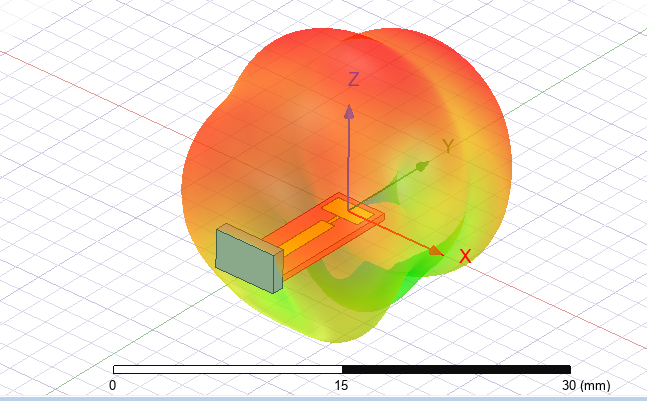
\includegraphics[width=\linewidth,height=2.08cm,keepaspectratio]{AntennaAndPattern.PNG}
  \begin{columns}[T,onlytextwidth]
    \column{0.57\textwidth}
      \centering
      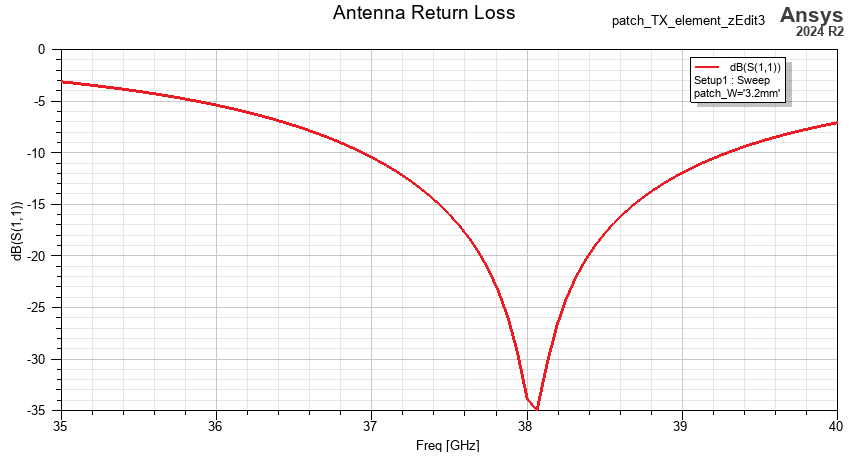
\includegraphics[width=\linewidth,height=1.80cm,keepaspectratio]{AntennaPatchReturnLoss.png}
    \column{0.41\textwidth}
      \centering
      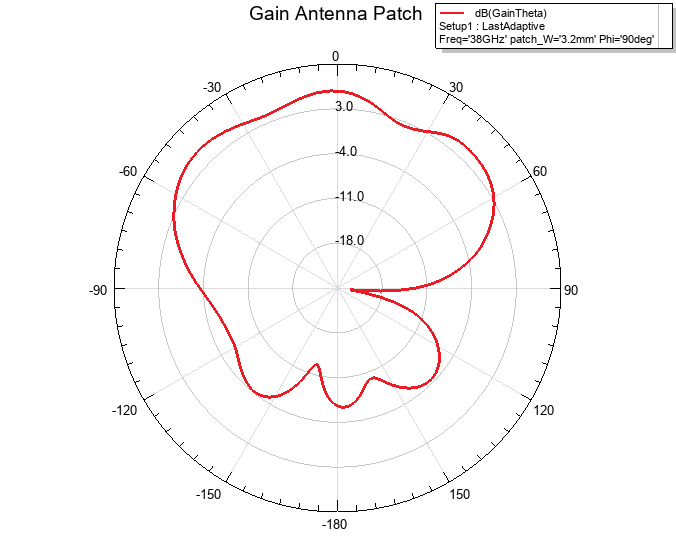
\includegraphics[width=\linewidth,height=1.80cm,keepaspectratio]{GainThetaAntennaPatch.png}
  \end{columns}
  \ThesisFigureCaption{2-1}{Patch geometry and 3D pattern, return loss, and
  $\phi=90^\circ$ gain cut at 38~GHz.}
\end{columns}
\note{
  \begin{itemize}
    \item Figure 2-1 combines the physical antenna model, its
          impedance match, and the 38~GHz angular response.
    \item The return-loss minimum occurs near 38.1~GHz at approximately
          $-35$~dB. The plotted $-10$-dB band is approximately
          36.9--39.5~GHz, so 38~GHz is well matched.
    \item The 3D and $\phi=90^\circ$ cuts show a dominant forward response with
          weaker back radiation, suitable for illuminating the transmitarray.
    \item This physical patch belongs to the lens characterization. The
          controlled Chapter~3 trajectory study intentionally uses ideal
          isotropic TX elements.
  \end{itemize}
}
\end{frame}


\begin{frame}[t]{Metasurface Unit Cell: Architecture and Floquet Setup}
\begin{columns}[T,onlytextwidth]
  \column{0.39\textwidth}
  \centering
  \begin{columns}[T,onlytextwidth]
    \column{0.34\textwidth}
      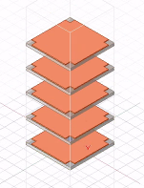
\includegraphics[height=1.72cm]{Unitcell_Design.png}
    \column{0.63\textwidth}
      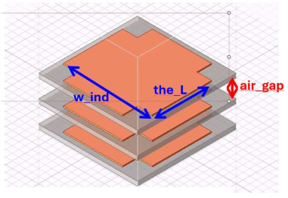
\includegraphics[width=\linewidth,height=1.72cm,keepaspectratio]{Unitcell_Design_geometry.png}
  \end{columns}
  \ThesisFigureCaption{2-2}{Five-layer unit cell and swept geometry.}

  \vspace{0cm}
  \scriptsize\raggedright
  \begin{itemize}
    \setlength{\itemsep}{-0.12em}
    \item \textbf{Material:} Rogers RT/duroid 5880LZ,
          $\varepsilon_r=2.2$, substrate thickness $h=0.787$~mm.
    \item \textbf{Stack:} five patterned layers with
          $g_{\mathrm{air}}=1$~mm gaps.
    \item Swept $L$ and $W_{\mathrm{ind}}$ control transmission magnitude and
          phase.
  \end{itemize}

  \column{0.57\textwidth}
  \centering
  \begin{columns}[T,onlytextwidth]
    \column{0.24\textwidth}
      \centering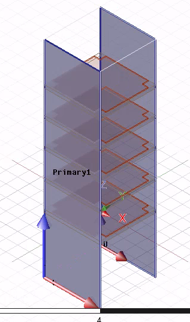
\includegraphics[width=\linewidth,height=2.70cm,keepaspectratio]{FloqBoundary-1.png}
      \SlideCaption{periodic 1}
    \column{0.24\textwidth}
      \centering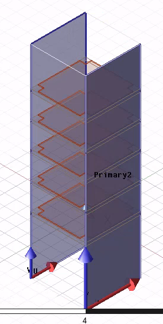
\includegraphics[width=\linewidth,height=2.70cm,keepaspectratio]{FloqBoundary-2.png}
      \SlideCaption{periodic 2}
    \column{0.24\textwidth}
      \centering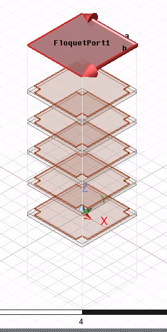
\includegraphics[width=\linewidth,height=2.70cm,keepaspectratio]{FloqPort-1.png}
      \SlideCaption{port 1}
    \column{0.24\textwidth}
      \centering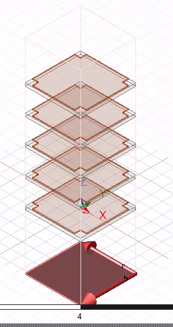
\includegraphics[width=\linewidth,height=2.70cm,keepaspectratio]{FloqPort-2.png}
      \SlideCaption{port 2}
  \end{columns}
  \vspace{0cm}
  \MethodNote{\textbf{Figure 2-3:} periodic boundaries + Floquet
  ports emulate plane-wave excitation and generate the transmission library.}
\end{columns}
\note{
  \begin{itemize}
    \item I implement Kanghyeok Lee's design for unitcell, his paper is Broadband metasurface superstrate for polarization-independent wave focusing and gain enhancement at Ka-band(28-32Ghz)
    \item it can using on vertical and horizontal polarization. But in this thesis, we only use vertical polarization
    \item The implemented unit cell uses Rogers RT/duroid 5880LZ with a
          substrate thickness of 0.787~mm and relative permittivity
          $\varepsilon_r=2.2$; its five patterned layers are separated by
          1~mm air gaps.
    \item This unit cell design is the most flexible unit cell design that i found so far.
    \item The adopted topology was reported as a broadband,
          polarization-independent Ka-band design \cite{Lee2022}; this thesis
          uses the vertical-polarization response.
  \end{itemize}
}
\end{frame}


\begin{frame}[t]{Transmission Library: Efficiency and Phase Coverage}
\begin{columns}[T,onlytextwidth]
  \column{0.35\textwidth}
  \tiny
  \begin{align*}
    |S_{11}|^2+|S_{21}|^2+P_{\mathrm{loss}}&=1,\\
    \eta_{\mathrm{trans}}=|S_{21}|^2&=10^{S_{21,\mathrm{dB}}/10},\\[-2pt]
    \eta_{\mathrm{refl}}=|S_{11}|^2&=10^{S_{11,\mathrm{dB}}/10}.
  \end{align*}
  \begin{block}{Selection at 38~GHz}
    \centering
    \large $S_{21}>-5\,\mathrm{dB}$\\[-1pt]
    \scriptsize $P_T>31.6\%$
  \end{block}
  \scriptsize
  \textbf{Accepted library:} 324 geometries with an approximately
  $258^\circ$ wrapped-phase span at 38~GHz. This broadens design flexibility,
  but does not provide complete $360^\circ$ coverage.

  \column{0.61\textwidth}
  \centering
  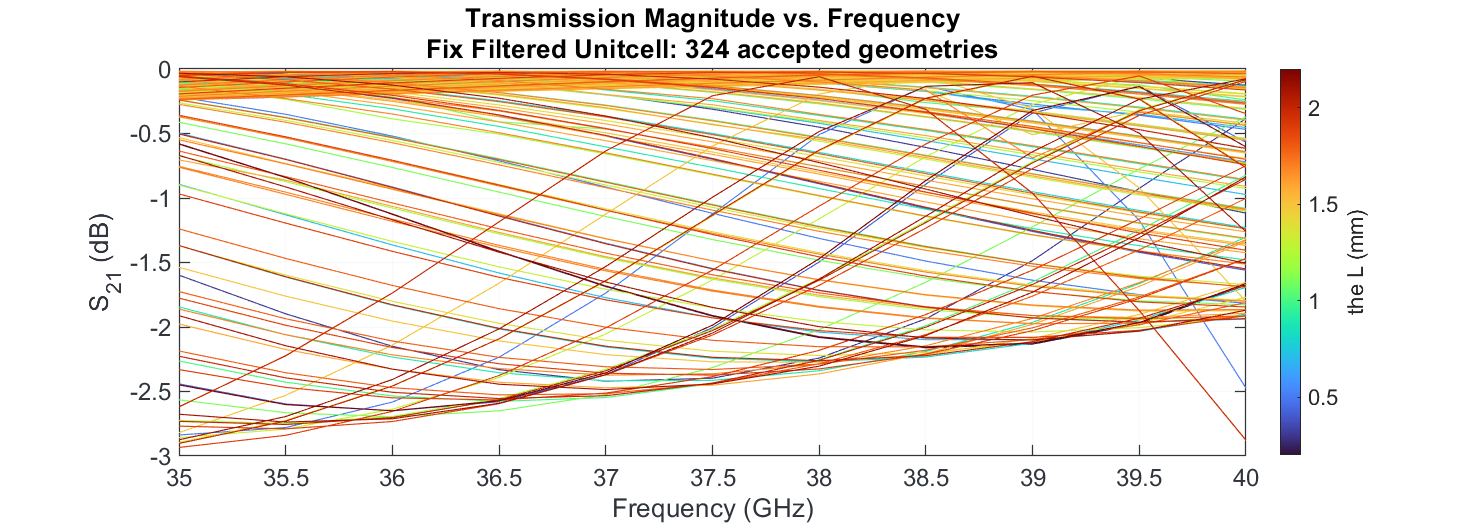
\includegraphics[width=\linewidth,height=2.20cm,keepaspectratio]{UnitCellProfile_Magnitude_Accepted.png}
  \vspace{0.05cm}
  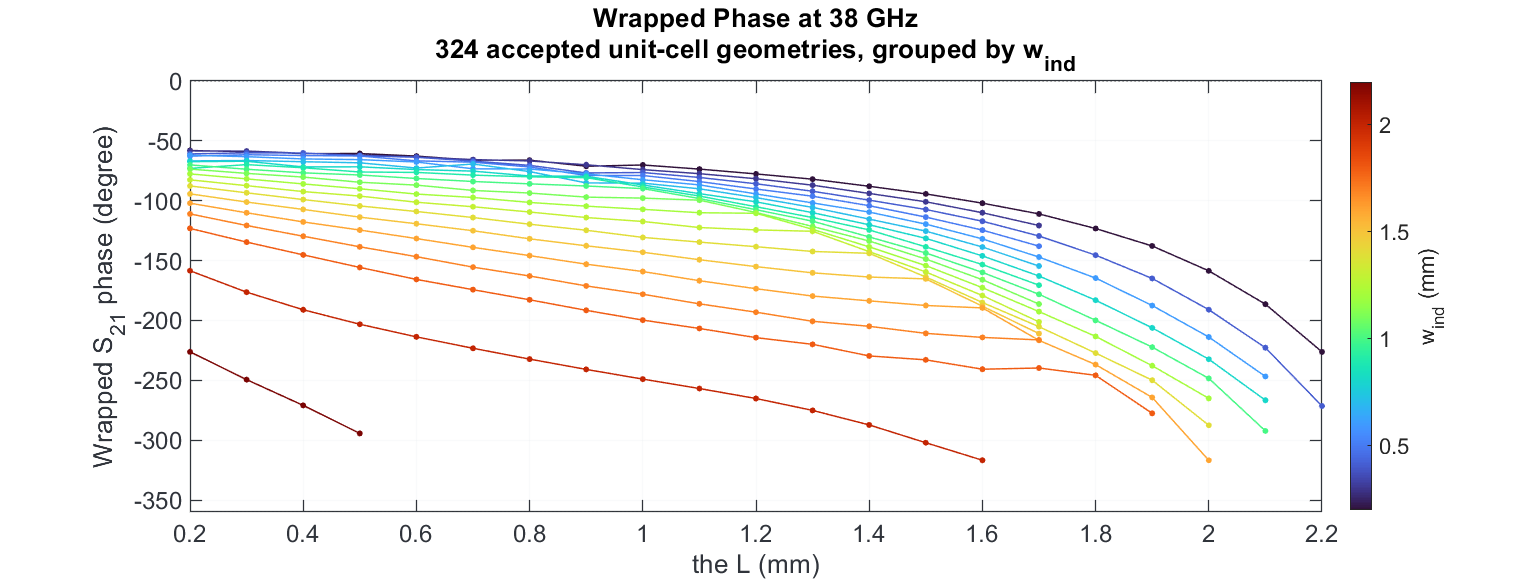
\includegraphics[width=\linewidth,height=2.20cm,keepaspectratio]{UnitCellProfile_PhaseAt38GHz_Accepted.png}
  \ThesisFigureCaption{2-4}{Magnitude and wrapped phase of the 324 geometries
  accepted using $S_{21}>-5$~dB at 38~GHz.}
\end{columns}
% % \Takeaway{Use only phase states that also satisfy the transmission-efficiency
% criterion.}
\SourceNote{Chapter 2: Metasurface Unit-Cell Design}
\note{
  \begin{itemize}
    \item Figure 2-4 shows only the 324 geometries that satisfy
          $S_{21}>-5$~dB at the 38~GHz design frequency.
    \item At the threshold, the transmitted-power fraction is
          $10^{-5/10}=0.316$, so every retained state transmits more than 31.6\%.
    \item The wrapped phase extends from approximately $-58^\circ$ to
          $-316^\circ$, giving a span of about $258^\circ$.
    \item The correct claim is broader design flexibility, not complete
          $360^\circ$ phase coverage. Residual phase quantization remains.
  \end{itemize}
}
\end{frame}


\begin{frame}[t]{From Required Phase to the Realized $20\times20$ Lens}
\begin{columns}[T,onlytextwidth]
  \column{0.43\textwidth}
  \scriptsize
  \begin{equation*}
    \begin{aligned}
      d(x,y)&=\sqrt{(x-x_f)^2+(y-y_f)^2+f^2},\\
      \phi(x,y)&=\frac{2\pi}{\lambda_0}\,[d(x,y)-f]+\phi_{\mathrm{init}}.
    \end{aligned}
  \end{equation*}
  \scriptsize
  The phase mask compensates path-length differences; the finite cell library
  discretizes the continuous profile \cite{Al-Joumayly2011}.

  \vspace{0cm}
  {\scriptsize
  \renewcommand{\arraystretch}{0.76}
  \begin{tabularx}{\linewidth}{@{}Xr@{}}
    \toprule
    \textbf{Parameter} & \textbf{Value}\\
    \midrule
    Array size & $20\times20$\\
    Aperture & $44.24\times44.24$~mm$^2$\\
    Layers & 5\\
    Target focal distance & 30~mm\\
    Realized focus & $\approx14$~mm\\
    \bottomrule
  \end{tabularx}}

  \column{0.27\textwidth}
  \centering
  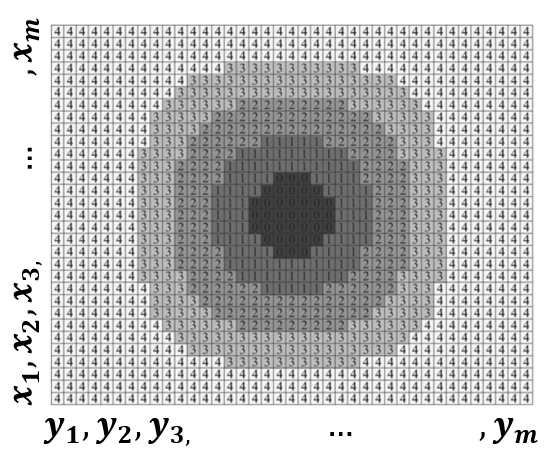
\includegraphics[height=1.70cm,width=\linewidth,keepaspectratio]{AntennaLensFrontView.PNG}
  \ThesisFigureCaption{2-5}{Discrete radial state map.}
  \vspace{0.08cm}
  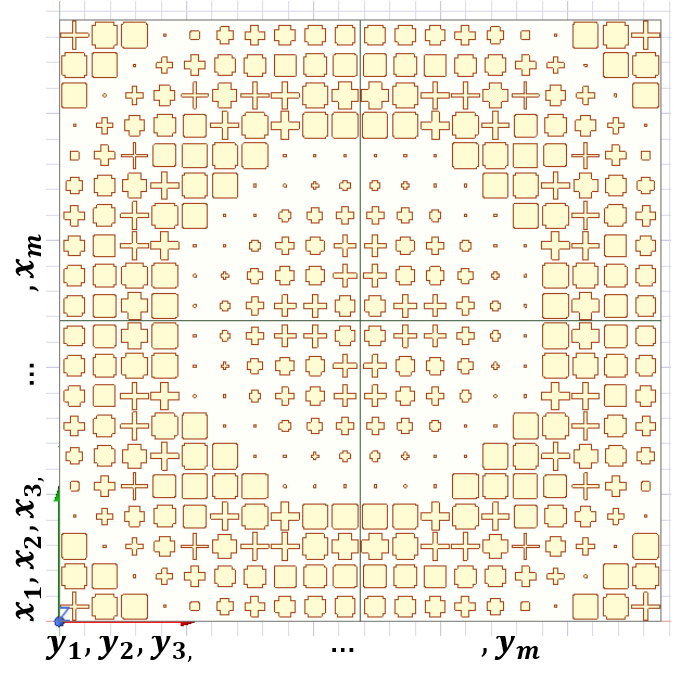
\includegraphics[height=1.70cm,width=\linewidth,keepaspectratio]{AntennaLensTopView_edited.PNG}
  \ThesisFigureCaption{2-6}{Physical transmitarray layout.}

  \column{0.26\textwidth}
  \centering
  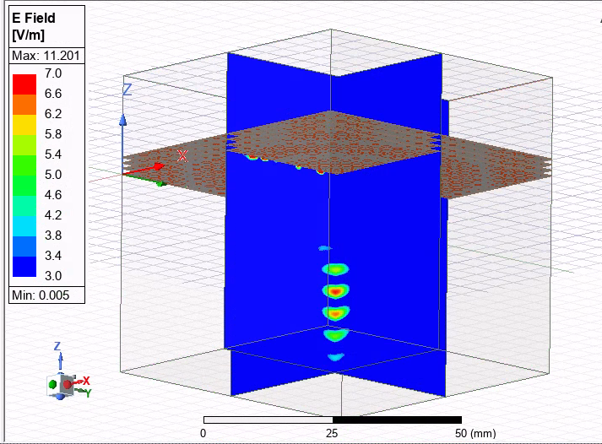
\includegraphics[height=4.00cm,width=\linewidth,keepaspectratio]{AntennaLens20x20_VerifFocalPoint.png}
  \ThesisFigureCaption{2-7}{Axial E-field contraction.}
\end{columns}
\Takeaway{The realized focus is $\approx14$~mm versus the 30~mm target; the
thesis attributes this offset to phase quantization.}
\note{
  \begin{itemize}
    \item And after found out unit-cell profil, we design the lens with 20x20 element, and the target focal distance is 30mm, but the realized focal distance is 14mm, because of phase quantization
  \end{itemize}
}
\end{frame}


\begin{frame}[t]{Angular Focusing Traces a Focal Arc}
\centering
\begin{tabular}{@{}ccccc@{}}
  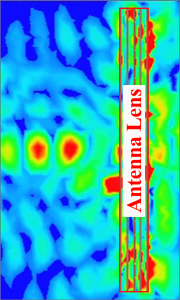
\includegraphics[height=3.68cm]{FocalCharacter_0deg.png} &
  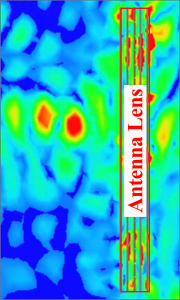
\includegraphics[height=3.68cm]{FocalCharacter_m15degdeg.png} &
  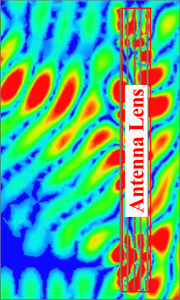
\includegraphics[height=3.68cm]{FocalCharacter_m30deg.png} &
  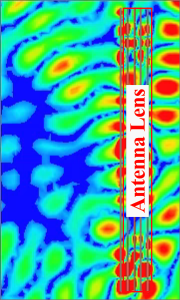
\includegraphics[height=3.68cm]{FocalCharacter_m45deg.png} &
  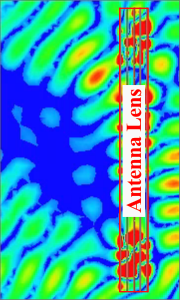
\includegraphics[height=3.68cm]{FocalCharacter_m60deg.png} \\
  {\scriptsize $0^\circ$} & {\scriptsize $-15^\circ$} &
  {\scriptsize $-30^\circ$} & {\scriptsize $-45^\circ$} &
  {\scriptsize $-60^\circ$}
\end{tabular}
\ThesisFigureCaption{2-8}{Focal-plane response for incidence angles from
$0^\circ$ to $-60^\circ$.}

\vspace{0.08cm}
\begin{columns}[T,onlytextwidth]
  \column{0.48\textwidth}
  \MethodNote{The energy peak shifts laterally while remaining at approximately
  the same radial distance: a \textbf{focal arc}.}
  \column{0.48\textwidth}
  \CautionNote{Focus is sharpest near $0^\circ$ and $-15^\circ$; diffuse peaks
  and sidelobes increase toward $-60^\circ$.}
\end{columns}
\SourceNote{Chapter 2: Focal Characteristics}
\note{
  \begin{itemize}
    \item This Near-field patterns Confirm the angle-dependent steering, and the energy peak shifts laterally while remaining at approximately the same radial distance: a focal arc
    \item Focus is sharpest near $0^\circ$ and $-15^\circ$; diffuse peaks and sidelobes increase toward $-60^\circ$. it also spoiled by Al-Joumayly2011 in his paper on incident at 45degree, the focus is not sharp, and the sidelobe is very high
  \end{itemize}
}
\end{frame}


\begin{frame}[t]{3D Far-Field Patterns Confirm Angle-Dependent Steering}
\centering
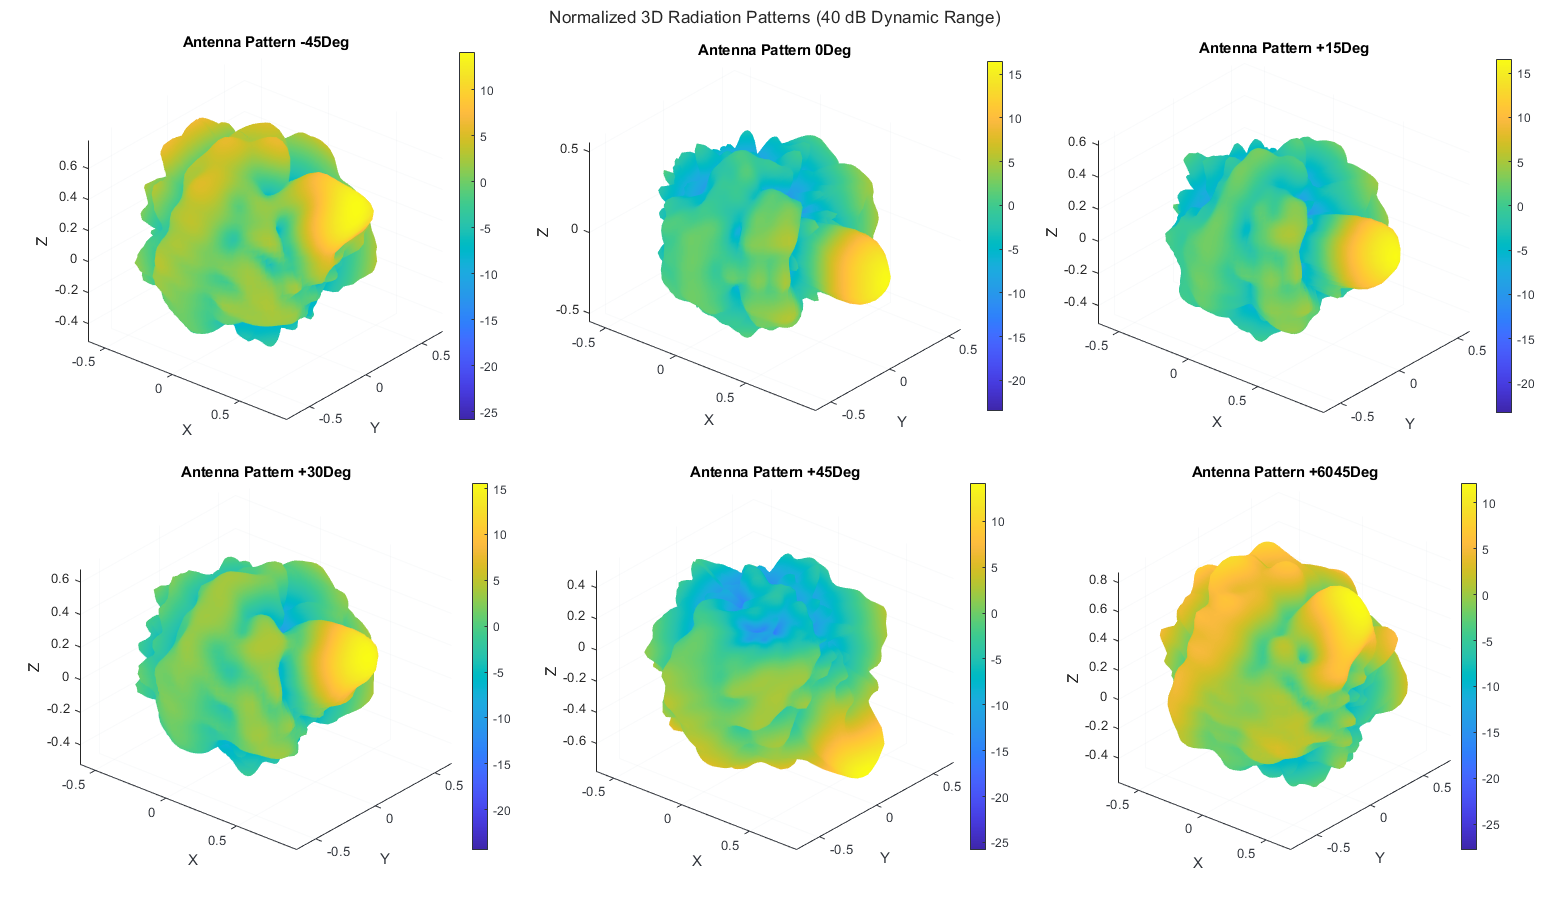
\includegraphics[width=0.74\linewidth,height=4.75cm,keepaspectratio]
  {AntennaPatternWithLens.png}
\ThesisFigureCaption{2-10}{Normalized 3D patterns for six representative
lens-assisted RX states at 38~GHz.}
\begin{columns}[T,onlytextwidth]
  \column{0.48\textwidth}
  \MethodNote{Boresight and moderate-angle states retain a comparatively
  distinct dominant lobe as the focal-plane state changes.}
  \column{0.48\textwidth}
  \CautionNote{The widest-angle patterns are less regular; the vertical cut is
  used to quantify peak direction, gain, ripple, and secondary lobes.}
\end{columns}
\note{
  \begin{itemize}
    \item Figure 2-10 replaces the previous 3D-pattern asset.
    \item Changing the focal-plane RX state displaces the dominant radiation
          region and changes the secondary-lobe structure.
    \item The boresight and moderate-angle states show clearer dominant beams;
          the widest-angle states are more irregular, consistent with the
          off-axis focal spreading in Figure 2-8.
    \item Do not quote the previous low-90\% efficiency claim here; that metric
          is not displayed in the updated draft figures.
    \item Figure 2-11 provides the quantitative X--Z-plane comparison.
  \end{itemize}
}
\end{frame}


\begin{frame}[t]{Vertical Cuts Quantify RX Lens Beam Steering}
\centering
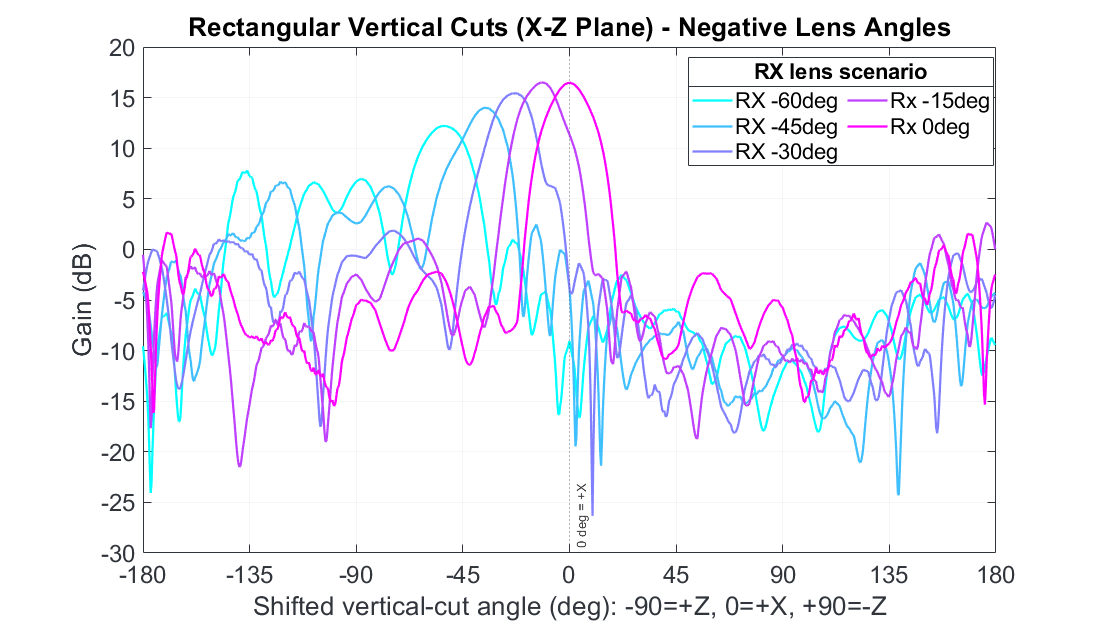
\includegraphics[width=0.72\linewidth,height=4.55cm,keepaspectratio]
  {RXAntennaRadiationPattern.png}
\ThesisFigureCaption{2-11}{Rectangular X--Z-plane gain cuts for RX states
$0^\circ,-15^\circ,-30^\circ,-45^\circ,-60^\circ$.}

\begin{columns}[T,onlytextwidth]
  \column{0.48\textwidth}
  \MethodNote{The main-lobe peak shifts from approximately $0^\circ$ for RX
  $0^\circ$ toward approximately $-55^\circ$ for RX $-60^\circ$.}
  \column{0.48\textwidth}
  \CautionNote{Larger steering offsets also produce stronger secondary lobes;
  beam direction and sidelobe structure must be assessed together.}
\end{columns}
\note{
  \begin{itemize}
    \item This rectangular plot isolates the vertical X--Z-plane response and
          makes the pointing direction easier to compare than in the 3D view.
    \item Figure 2-11 uses the shifted-angle convention
          $-90^\circ=+Z$, $0^\circ=+X$, and $+90^\circ=-Z$.
    \item The $0^\circ$ scenario peaks near the $+X$ reference direction. As the
          selected RX lens state changes through $-15^\circ$, $-30^\circ$,
          $-45^\circ$, and $-60^\circ$, the main lobe moves progressively toward
          approximately $-55^\circ$.
    \item Peak gain decreases from about 16~dB near boresight and the
          moderate-angle states to approximately 12~dB for RX $-60^\circ$.
    \item Secondary lobes and nulls become more pronounced away from boresight,
          consistent with the less-sharp focal patterns observed at larger
          steering offsets.
    \item This angle-dependent response is later imported into the channel
          simulations as a distinct RX pattern for each lens branch.
  \end{itemize}
}
\end{frame}


\subsection{Channel Formulation and Metrics}

\begin{frame}[t]{Canonical $3\times3$ Angular-Domain MIMO Channel}
\begin{columns}[T,onlytextwidth]
  \column{0.47\textwidth}
  \small
  \begin{align*}
    \mathbf y(f)&=\mathbf H(f)\mathbf x(f)+\mathbf n(f)
                   \quad\text{\cite{Tse2005}},\\
    \mathbf H(f)&=
    \begin{bmatrix}
      H_{11} & H_{12} & H_{13}\\
      H_{21} & H_{22} & H_{23}\\
      H_{31} & H_{32} & H_{33}
    \end{bmatrix}.
  \end{align*}
  \scriptsize
  \begin{tabular}{@{}cll@{}}
    \toprule
    \textbf{Pair} & \textbf{Angle} & \textbf{Role}\\
    \midrule
    $\mathrm{rx}_1,\mathrm{tx}_1$ & $0^\circ$ & boresight\\
    $\mathrm{rx}_2,\mathrm{tx}_2$ & $+45^\circ$ & positive-angle\\
    $\mathrm{rx}_3,\mathrm{tx}_3$ & $-45^\circ$ & negative-angle\\
    \bottomrule
  \end{tabular}
  \vspace{0.25cm}

  $H_{ii}$: direction-matched link.\par
  $H_{ij},\ i\neq j$: cross-angular coupling \cite{Challita2022}.

  \column{0.49\textwidth}
  \centering
  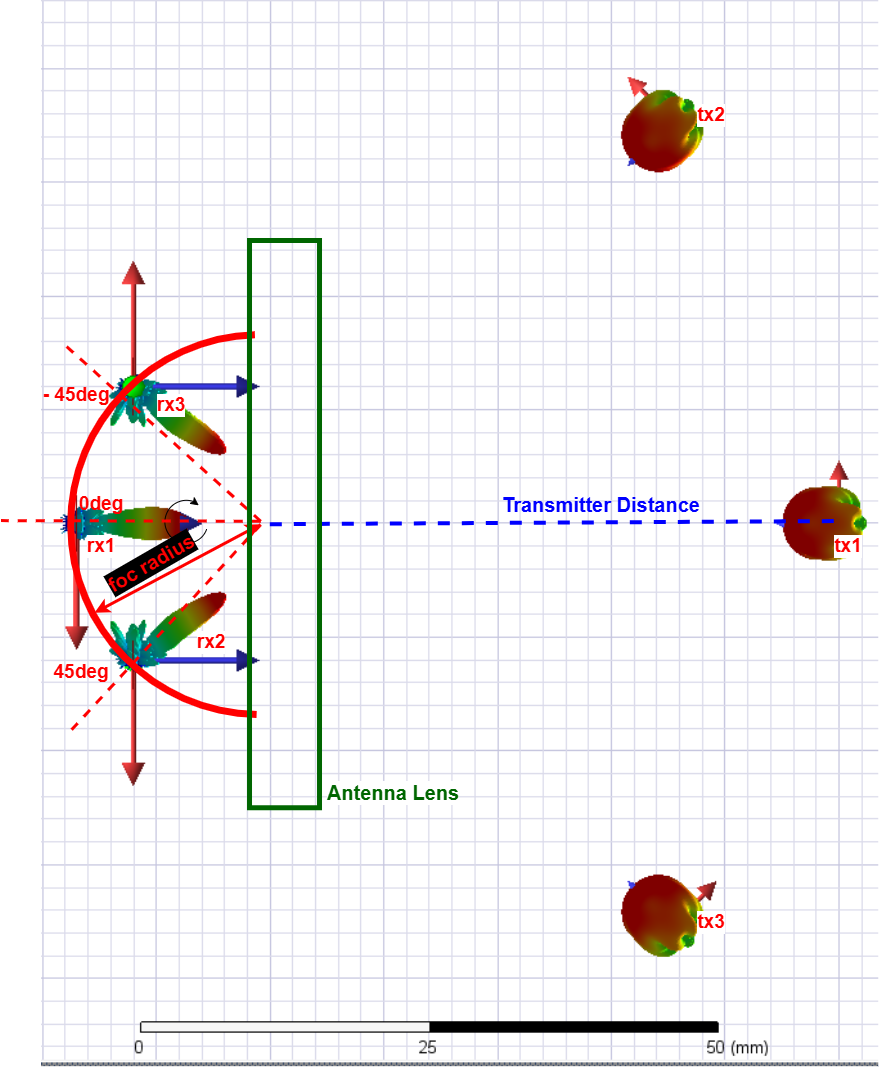
\includegraphics[height=4.60cm,width=\linewidth,keepaspectratio]
    {SetupEnvirontment_SBR_WithLens_TopDetails.PNG}
  \ThesisFigureCaption{2-15}{Focal-arc RX positions and matched TX directions.}
\end{columns}
% \Takeaway{The lens strengthens $H_{ii}$ while suppressing cross-angular
% $H_{ij}$, $i\neq j$.}
\note{
  \begin{itemize}
    \item This is CSI formulation, and the channel matrix is 3x3, and the diagonal element is direction-matched link, and the off-diagonal element is cross-angular coupling
    \item The lens strengthens $H_{ii}$ while suppressing cross-angular $H_{ij}$, $i\neq j$.
    \item Takeaway: The lens strengthens $H_{ii}$ while suppressing cross-angular $H_{ij}$, $i\neq j$.
  \end{itemize}
}
\end{frame}


\begin{frame}[t]{Different Solvers, One Effective CSI Convention}
\scriptsize
\setlength{\abovedisplayskip}{0.25ex}
\setlength{\belowdisplayskip}{0.35ex}
\begin{columns}[T,onlytextwidth]
  \column{0.318\textwidth}
  \begin{block}{HFSS SBR+}
    {\tiny
    \begin{align*}
      H_{ij}^{\mathrm{HFSS}}(f)
      &=S(\mathrm{rx}_i,\mathrm{tx}_j;f)\\[-2pt]
      &=\left.\frac{b_i(f)}{a_j(f)}\right|_{a_{k\neq j}=0}.
      \tag{2.15}
    \end{align*}}
    Rays undergo reflection/transmission; physical-optics fields are coherently
    projected onto the RX polarized-gain vector.
  \end{block}

  \column{0.318\textwidth}
  \begin{block}{HFSS Hybrid}
    {\tiny
    \begin{align*}
      &\nabla\!\times\!(\mu_r^{-1}\nabla\!\times\!\mathbf E)\\[-2pt]
      &\quad-k_0^2\varepsilon_r\mathbf E
      =-j\omega\mu_0\mathbf J_{\mathrm{exc}}
      \tag{2.28}\\[-1pt]
      \mathbf J_H&=\hat n\times\mathbf H_{\mathrm{FEM}},\\[-2pt]
      \mathbf M_H&=-\hat n\times\mathbf E_{\mathrm{FEM}}.
      \tag{2.32}
    \end{align*}}
    A Huygens surface couples the full-wave antenna--lens region to room-scale
    SBR+ propagation.
  \end{block}

  \column{0.318\textwidth}
  \begin{block}{Sionna-RT}
    {\tiny
    \begin{align*}
      h_{ij}(\tau)&=\sum_{\ell}\alpha_{ij,\ell}
      \delta(\tau-\tau_{ij,\ell})
      \tag{2.18}\\
      H_{ij}(f)&=\sum_{\ell}\alpha_{ij,\ell}
      e^{-j2\pi f\tau_{ij,\ell}}.
      \tag{2.19}
    \end{align*}}
    Resolved paths are coherently summed into the same canonical frequency-domain
    coefficient \cite{NVIDIACorporation2026,Tse2005}.
  \end{block}
\end{columns}

% \Takeaway{Each $H_{ij}$ is an effective end-to-end response. Its exact reference
% quantity is solver-specific, but its matrix role is common.}
\note{
  \begin{itemize}
    \item In this slide, we show the different solver, and the CSI formulation is different, but the role of CSI is the same
    \item Ansys HFSS uses S-parameters to represent the channel, and the S-parameter is the ratio of output voltage to input voltage, and the S-parameter is a complex number, so it can represent the amplitude and phase of the channel
    \item Sionna-RT uses the impulse response to represent the channel, and the impulse response is the sum of the multipath components, and the impulse response is a complex number, so it can represent the amplitude and phase of the channel
    \item The HFSS Hybrid uses FEM to solve the antenna and lens region, and then uses SBR+ to solve the room, and then uses Huygens surface to couple the two regions, and then uses S-parameters to represent the channel
    \item The takeaway is that each $H_{ij}$ is an effective end-to-end response. Its exact reference quantity is solver-specific, but its matrix role is common.
    \item Takeaway: Each $H_{ij}$ is an effective end-to-end response. Its exact reference quantity is solver-specific, but its matrix role is common.
  \end{itemize}
}
\end{frame}


\begin{frame}[t]{Metrics Separate Link Gain from Spatial-Mode Quality}
\scriptsize
\setlength{\abovedisplayskip}{0.35ex}
\setlength{\belowdisplayskip}{0.45ex}
\begin{columns}[T,onlytextwidth]
  \column{0.49\textwidth}
  \begin{block}{SVD and mode balance}
    {\tiny
    \begin{align*}
      \mathbf H&=\mathbf U\boldsymbol\Sigma\mathbf V^H,
      \quad\boldsymbol\Sigma=\operatorname{diag}(\sigma_1,\sigma_2,\sigma_3)
      \tag{2.21}\\[-1pt]
      \kappa&=\frac{\sigma_1}{\sigma_3}\tag{2.23}\\[-1pt]
      p_i&=\frac{\sigma_i^2}{\sum_k\sigma_k^2}\tag{2.24}\\[-1pt]
      r_{\mathrm{eff}}&=\exp\!\left(-\sum_i p_i\ln p_i\right)\tag{2.25}
    \end{align*}}
    Better balance: $\kappa\rightarrow1$ and $r_{\mathrm{eff}}\rightarrow3$.
  \end{block}

  \begin{block}{Spatial correlation}
    \begin{equation*}
      \mathbf R_{\mathrm{RX}}=\mathbf D_{\mathrm{RX}}^{-1/2}
      \mathbf H\mathbf H^H\mathbf D_{\mathrm{RX}}^{-1/2}
      \tag{2.26}
    \end{equation*}
    with the analogous TX-side expression. Lower mean off-diagonal magnitude is
    better.
  \end{block}

  \column{0.49\textwidth}
  \begin{block}{Equal-power capacity at 20~dB}
    \begin{align*}
      C=\sum_{i=1}^{3}\log_2\!\left(1+\frac{\rho}{N_T}\sigma_i^2\right)
      &\quad\mathrm{bps/Hz},\tag{2.27}\\[-2pt]
      \rho&=100.
    \end{align*}
  \end{block}

  \begin{block}{Two complementary channel views}
    \begin{equation*}
      \widetilde{\mathbf H}=\frac{\mathbf H}{\lVert\mathbf H\rVert_F}
      \tag{2.22}
    \end{equation*}
    \textbf{Raw $\mathbf H$:} link budget + spatial structure.\par
    \textbf{Normalized $\widetilde{\mathbf H}$:} relative spatial-mode balance only.
    \par\smallskip
    \textbf{Invariant:} $\kappa$ and $r_{\mathrm{eff}}$.
    \textbf{Scale-sensitive:} capacity.
  \end{block}
\end{columns}
\note{
  \begin{itemize}
    \item In this slide How MIMO channel quality metrics are defined, and how they separate link gain from spatial-mode quality
    \item The SVD and mode balance, the spatial correlation, and the equal-power capacity
    \item The two complementary channel views, the raw H and the normalized H
  \end{itemize}
}
\end{frame}


\subsection{Simulation and Cross-Validation}

\begin{frame}[t]{Common Room Dimensions and Canonical Angular Setup}
\begin{columns}[T,onlytextwidth]
  \column{0.49\textwidth}
  \centering
  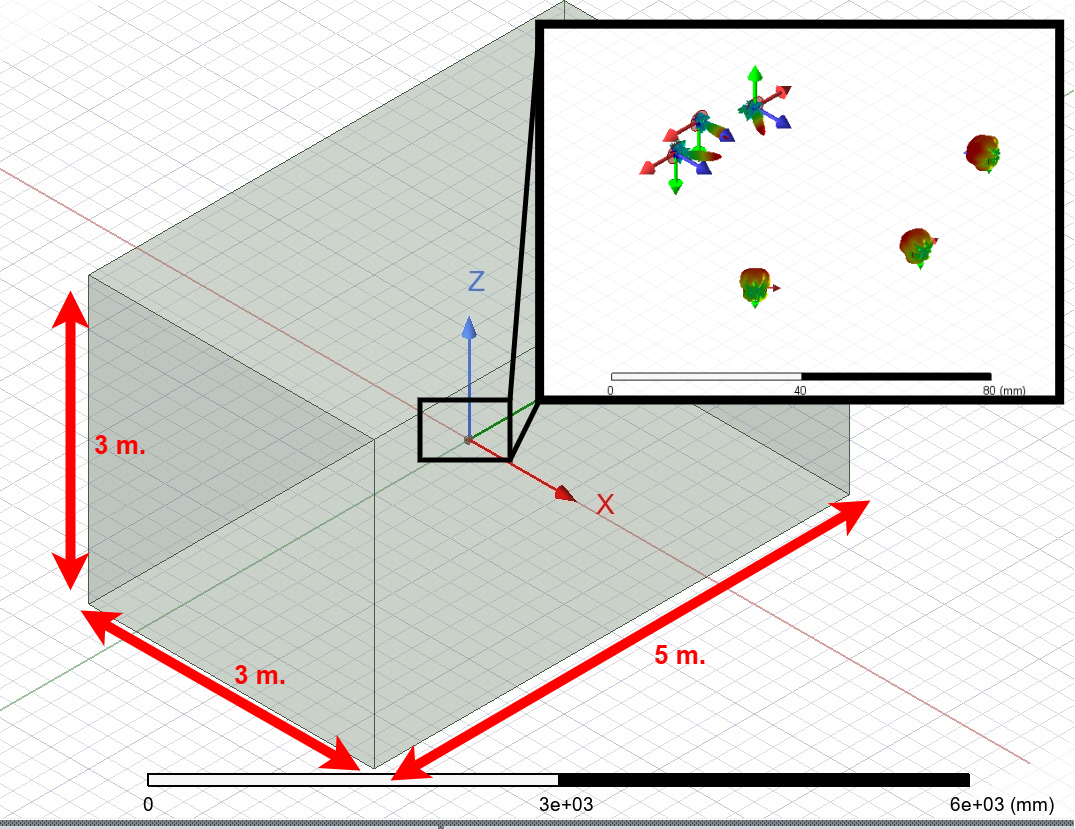
\includegraphics[width=\linewidth,height=3.35cm,keepaspectratio]{Room_SBR_withCloseup.png}
  \ThesisFigureCaption{2-12}{HFSS SBR+ room representation.}
  \column{0.49\textwidth}
  \centering
  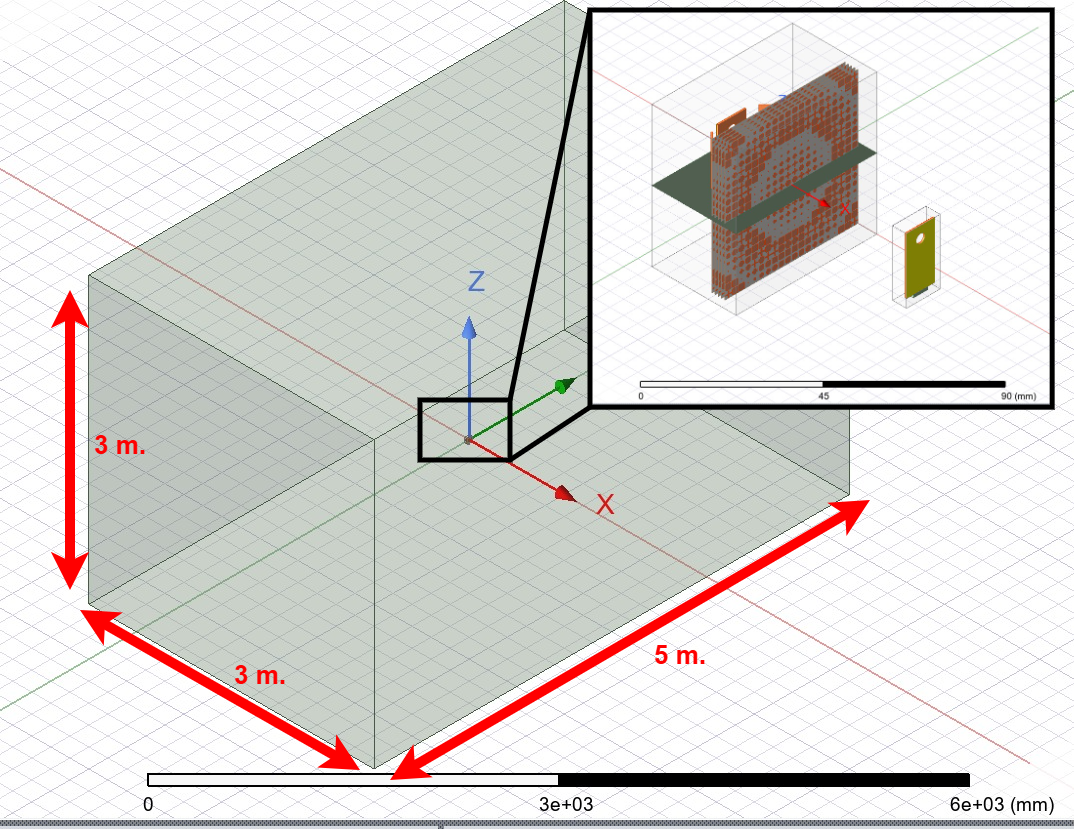
\includegraphics[width=\linewidth,height=3.35cm,keepaspectratio]{Room_withCloseup.png}
  \ThesisFigureCaption{2-13}{HFSS Hybrid room and explicit lens region.}
\end{columns}

\vspace{0.10cm}
\footnotesize
\begin{columns}[T,onlytextwidth]
  \column{0.32\textwidth}
  \textbf{Environment}\par
  $3\times5\times3$~m concrete room; LoS and reflected paths retained.
  \column{0.32\textwidth}
  \textbf{Angular sampling}\par
  RX/TX pairs at $0^\circ$, $+45^\circ$, $-45^\circ$; 37/38/39~GHz.
  \column{0.32\textwidth}
  \textbf{Paired experiment}\par
  Within each solver, geometry is fixed between lens/no-lens cases.
\end{columns}

% \Takeaway{Sionna-RT assembles the $3\times3$ matrix from three runs (one RX
% pattern per run), then applies the same channel indexing and metrics.}
\SourceNote{Chapter 2: HFSS Simulation Setup and Cross-Validation Setup}
\note{
  \begin{itemize}
    \item This is the simulation setup, and the room dimension is 3x5x3 meter, and the RX/TX pairs are at 0 degree, +45 degree, -45 degree, and the frequency is 37/38/39 GHz
    \item the scenario setup is the same for all three solvers, and the lens/no-lens cases are paired within each solver
    \item The takeaway is that Sionna-RT assembles the $3\times3$ matrix from three runs (one RX pattern per run), then applies the same channel indexing and metrics.    
    \item Takeaway: Sionna-RT assembles the $3\times3$ matrix from three runs (one RX pattern per run), then applies the same channel indexing and metrics.
  \end{itemize}
}
\end{frame}


\begin{frame}[t]{At 38~GHz, the Lens Concentrates Power on Matched Links}
\scriptsize
\centering
\begin{columns}[T,onlytextwidth]
  \column{0.32\textwidth}
  \centering\textbf{HFSS Hybrid}\par\vspace{0.15cm}
  \begin{tabular}{@{}ccc@{}}
    \HC{Blue!55}{\color{white}52.1} & \HC{Blue!4}{0.7} & \HC{Blue!4}{0.8}\\
    \HC{Blue!2}{$<0.1$} & \HC{Blue!25}{23.4} & \HC{Blue!4}{0.6}\\
    \HC{Blue!2}{$<0.1$} & \HC{Blue!4}{0.7} & \HC{Blue!23}{21.6}
  \end{tabular}
  \vspace{0.18cm}\par
  max cross term: $0.8\%$

  \column{0.32\textwidth}
  \centering\textbf{HFSS SBR+}\par\vspace{0.15cm}
  \begin{tabular}{@{}ccc@{}}
    \HC{Blue!65}{\color{white}62.2} & \HC{Blue!3}{0.3} & \HC{Blue!3}{0.2}\\
    \HC{Blue!5}{1.1} & \HC{Blue!19}{17.5} & \HC{Blue!2}{$<0.1$}\\
    \HC{Blue!5}{1.1} & \HC{Blue!2}{0.1} & \HC{Blue!19}{17.5}
  \end{tabular}
  \vspace{0.18cm}\par
  max cross term: $1.1\%$

  \column{0.32\textwidth}
  \centering\textbf{Sionna-RT}\par\vspace{0.15cm}
  \begin{tabular}{@{}ccc@{}}
    \HC{Blue!61}{\color{white}58.2} & \HC{Blue!3}{0.2} & \HC{Blue!3}{0.3}\\
    \HC{Blue!3}{0.2} & \HC{Blue!23}{21.1} & \HC{Blue!3}{0.2}\\
    \HC{Blue!3}{0.2} & \HC{Blue!3}{0.2} & \HC{Blue!21}{19.4}
  \end{tabular}
  \vspace{0.18cm}\par
  max cross term: $0.3\%$
\end{columns}

\vspace{0.55cm}
\begin{columns}[T,onlytextwidth]
  \column{0.48\textwidth}
  \MethodNote{\centering\textbf{With lens:} diagonal-dominant matrices across
  all solvers. Values above are normalized power shares (\%) at 38~GHz.}
  \column{0.48\textwidth}
  \CautionNote{\centering\textbf{Without lens:} power is much more diffuse;
  the direction-matched shares are only about 13--22\%.}
\end{columns}

% \Takeaway{The most solver-consistent physical effect is angular selectivity:
% matched links are reinforced while cross-directional coupling is suppressed.}
\SourceNote{Chapter 2: HFSS SBR+, HFSS Hybrid, and Sionna-RT Results}
\note{
  \begin{itemize}
    \item Showed the 3x3 channel matrix at 38GHz, and the diagonal element is direction-matched link, and the off-diagonal element is cross-angular coupling
    \item all solver showed that the lens concentrates power on matched links, and the max cross term is less than 1.1%
    \item So it can be concluded lens can improve the angular selectivity, and matched links are reinforced while cross-directional coupling is suppressed.
    \item takeaway: The most solver-consistent physical effect is angular selectivity: matched links are reinforced while cross-directional coupling is suppressed.
  \end{itemize}
}
\end{frame}


\begin{frame}[t]{Three-Solver MIMO Metrics at the 38~GHz Design Frequency}
\scriptsize
\setlength{\tabcolsep}{2.5pt}
\renewcommand{\arraystretch}{1.32}
\centering
\begin{tabular}{@{}lccccc@{}}
  \toprule
  \textbf{Solver} & $\boldsymbol{\kappa}$ & $\boldsymbol{r_{\mathrm{eff}}}$ &
  \textbf{Mean corr. RX/TX} & \textbf{Raw $C$} & \textbf{Normalized $C$}\\
  \midrule
  HFSS Hybrid & $4.42\!\rightarrow\!\mathbf{1.58}$ & $2.06\!\rightarrow\!\mathbf{2.73}$ &
  $.393/.561\!\rightarrow\!\mathbf{.085/.126}$ & $.38\!\rightarrow\!\mathbf{1.11}$ & $9.04\!\rightarrow\!\mathbf{10.46}$\\
  HFSS SBR+ & $6.25\!\rightarrow\!\mathbf{2.22}$ & $1.61\!\rightarrow\!\mathbf{2.36}$ &
  $.767/.767\!\rightarrow\!\mathbf{.213/.188}$ & $.60\!\rightarrow\!\mathbf{1.44}$ & $8.02\!\rightarrow\!\mathbf{9.92}$\\
  Sionna-RT & $2.06\!\rightarrow\!1.92$ & $2.60\!\rightarrow\!2.56$ &
  $.297/.335\!\rightarrow\!\mathbf{.177/.181}$ & $.32\!\rightarrow\!\mathbf{1.03}$ & $10.23\!\rightarrow\!10.20$\\
  \bottomrule
\end{tabular}

\vspace{0.25cm}
{\tiny Each entry is without lens $\rightarrow$ with lens. Capacities are in
bps/Hz at 20~dB. Bold marks the favorable endpoint when the change is substantive.}

\vspace{0.35cm}
\begin{columns}[T,onlytextwidth]
  \column{0.48\textwidth}
  \begin{block}{HFSS result}
    Both electromagnetic routes predict better conditioning, higher effective
    rank, lower correlation, and higher normalized capacity.
  \end{block}
  \column{0.48\textwidth}
  \begin{block}{Sionna-RT nuance}
    Decorrelation and raw capacity improve, but the already well-conditioned
    no-lens baseline leaves normalized capacity essentially unchanged.
  \end{block}
\end{columns}

% \Takeaway{All solvers support a link-budget benefit and lower correlation;
% improvement in relative spatial-mode balance is strongest in the HFSS models.}
\SourceNote{Chapter 2: Solver Results and Inter-Solver MIMO Comparison}
\note{
  \begin{itemize}
    \item then we show the MIMO metrics at 38GHz, and the diagonal element is direction-matched link, and the off-diagonal element is cross-angular coupling
    \item All solvers support a link-budget benefit and lower correlation; improvement in relative spatial-mode balance is strongest in the HFSS models.
    \item Takeaway: All solvers support a link-budget benefit and lower correlation; improvement in relative spatial-mode balance is strongest in the HFSS models.
  \end{itemize}
}
\end{frame}


\begin{frame}[t]{Spatial-Correlation Reduction Is Consistent Across Solvers}
\begin{columns}[T,onlytextwidth]
  \column{0.72\textwidth}
  \centering
  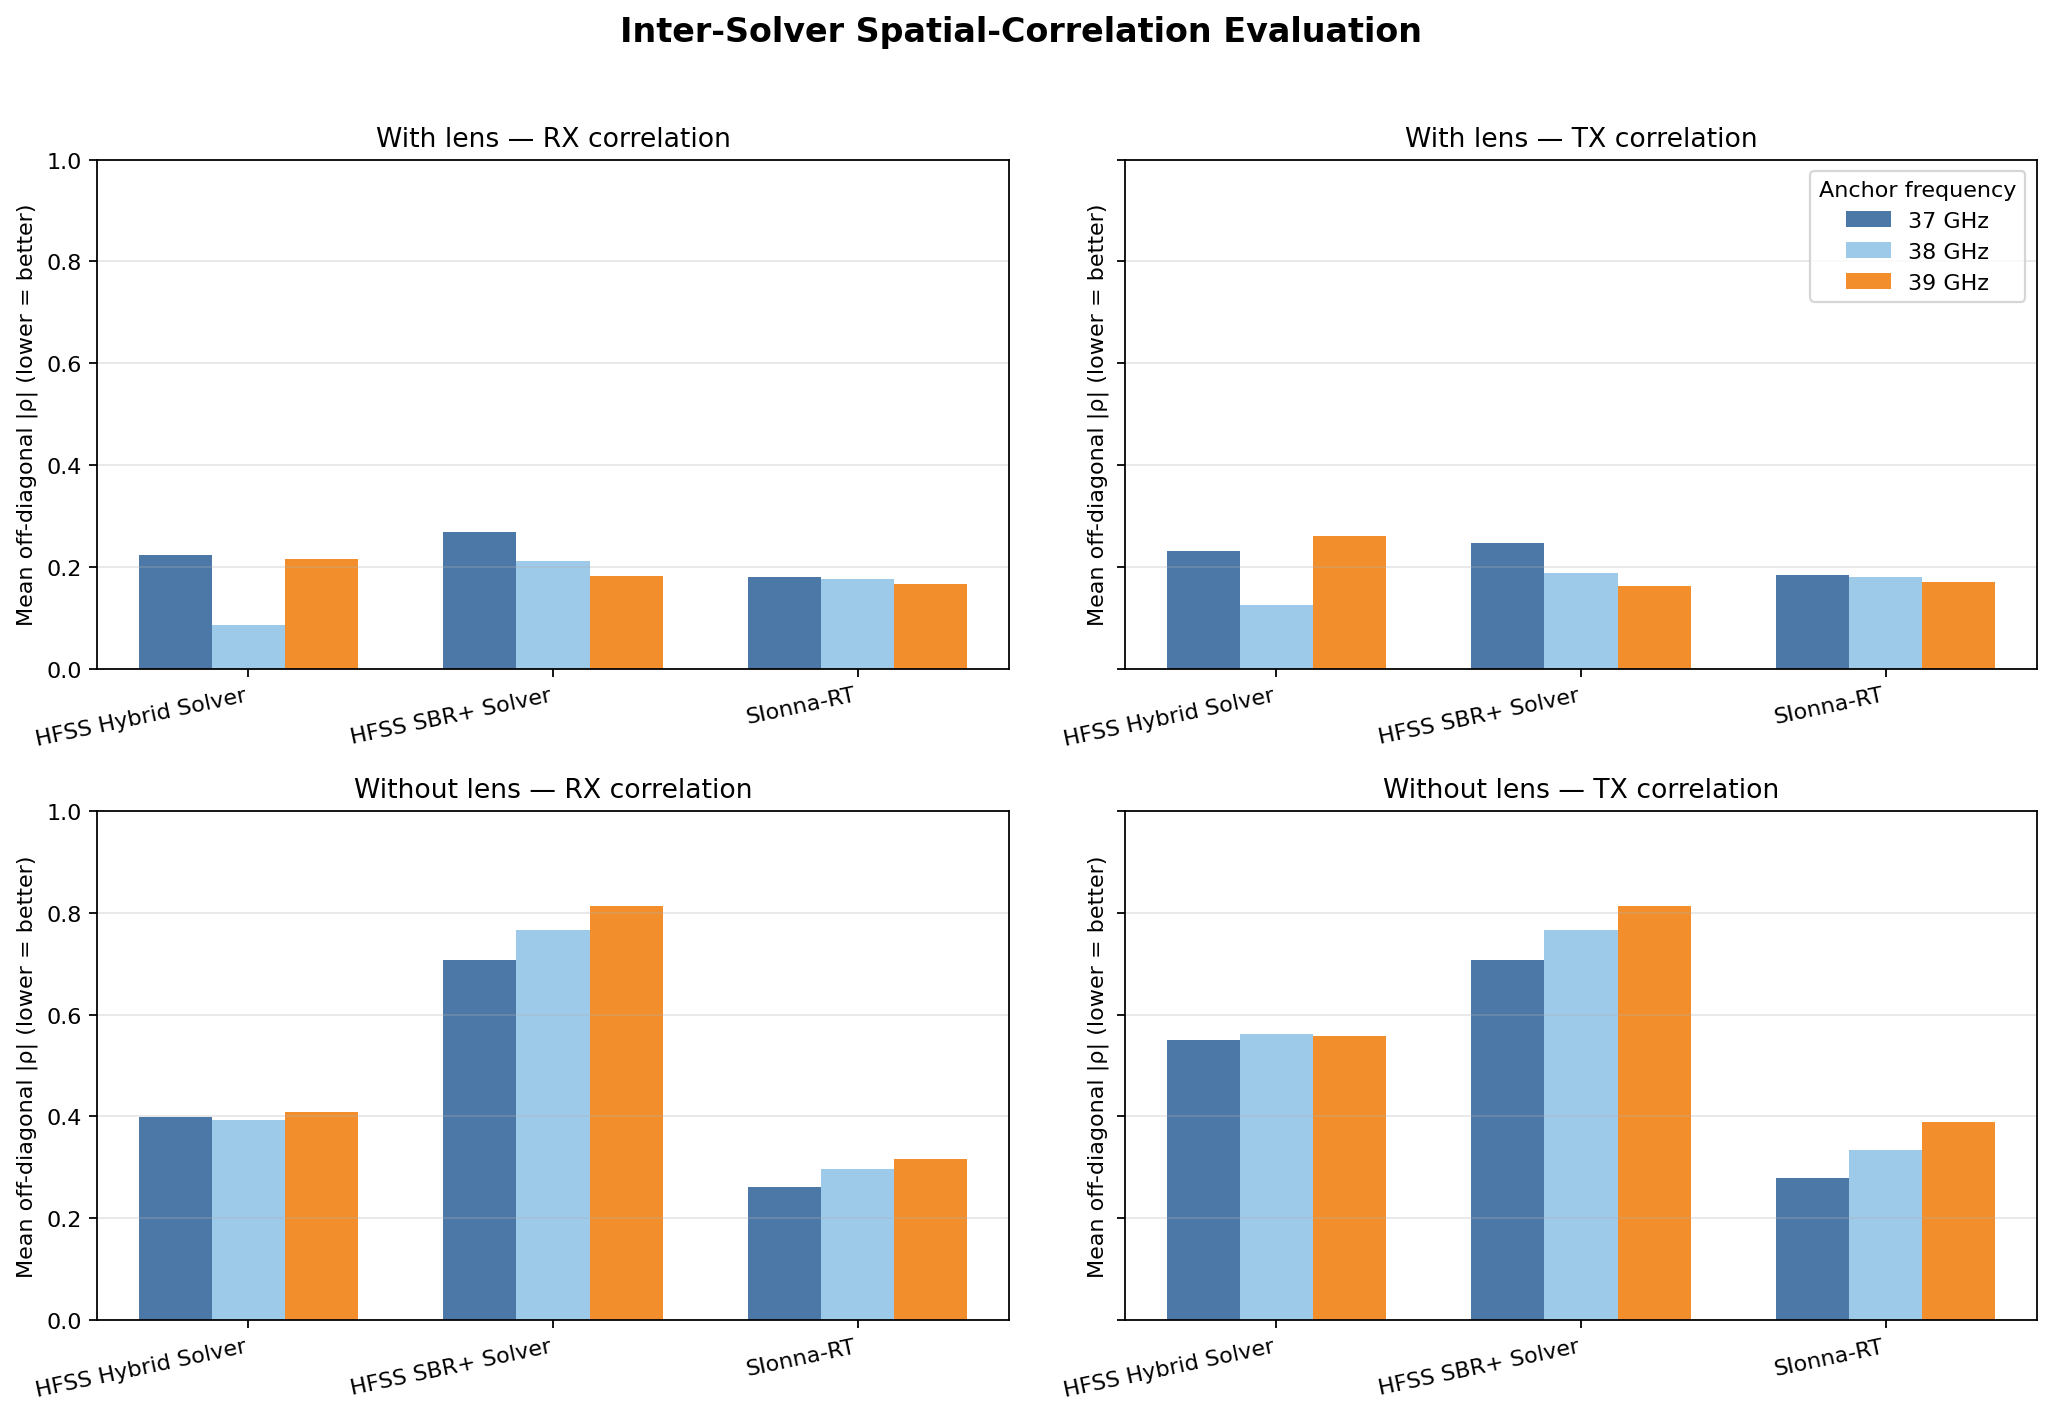
\includegraphics[width=\linewidth,height=5.15cm,keepaspectratio]
    {channel_comparison_results/mimo_spatial_correlation_evaluation.png}
  \ThesisFigureCaption{2-33}{Mean off-diagonal RX/TX correlation at 37, 38,
  and 39~GHz.}

  \column{0.24\textwidth}
  \scriptsize
  \begin{block}{With lens}
    All RX/TX means remain below approximately 0.27 at 37--39~GHz.
  \end{block}
  \begin{block}{Without lens}
    The baseline is solver-dependent, especially SBR+ versus Sionna-RT.
  \end{block}
  \begin{block}{Robust statement}
    Every solver predicts lower RX- and TX-side correlation at 38~GHz.
  \end{block}
\end{columns}
\SourceNote{Chapter 2: Spatial-Correlation Comparison}
\note{
  \begin{itemize}
    \item then we show the MIMO metrics at 38GHz, and the diagonal element is direction-matched link, and the off-diagonal element is cross-angular coupling
    \item All solvers support a link-budget benefit and lower correlation; improvement in relative spatial-mode balance is strongest in the HFSS models.
  \end{itemize}
}
\end{frame}


\begin{frame}[t]{Cross-Solver Agreement: Strong Trend, Solver-Specific Magnitude}
\begin{columns}[T,onlytextwidth]
  \column{0.55\textwidth}
  \footnotesize
  \begin{block}{Mean lens change, 37--39~GHz}
    \centering
    \begin{tabular}{@{}lrr@{}}
      \toprule
      \textbf{Solver} & \textbf{Diagonal} & \textbf{Off-diagonal}\\
      \midrule
      HFSS Hybrid & $+8.33$~dB & $-7.58$~dB\\
      HFSS SBR+ & $+5.33$~dB & $-7.86$~dB\\
      Sionna-RT & $+7.12$~dB & $-7.48$~dB\\
      \bottomrule
    \end{tabular}
  \end{block}

  \scriptsize
  \begin{itemize}
    \item All three solvers predict higher raw 20~dB capacity at 38~GHz.
    \item Absolute magnitudes and no-lens conditioning remain solver-specific.
    \item The only direction disagreements occur for
          $H(\mathrm{rx}_3,\mathrm{tx}_2)$ at 37 and 39~GHz.
  \end{itemize}

  \column{0.41\textwidth}
  \centering
  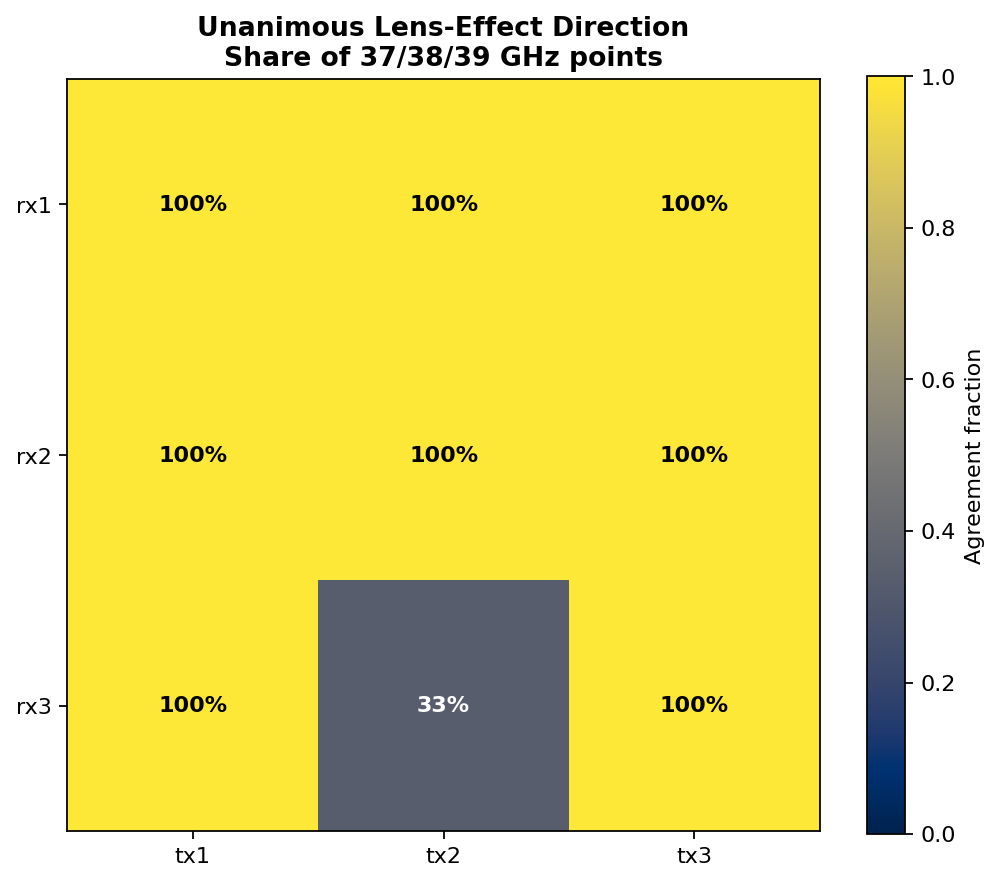
\includegraphics[width=\linewidth,height=4.25cm,keepaspectratio]
    {channel_comparison_results/lens_effect_direction_agreement.png}
  \ThesisFigureCaption{2-30}{Unanimous increase/decrease agreement by channel
  entry.}
\end{columns}

% \Takeaway{Lens-effect direction agrees at 25 of 27 link--frequency points
% (92.6\%).}
\SourceNote{Chapter 2: Cross-Solver Lens-Effect Comparison}
\note{
  \fontsize{7}{8}\selectfont
  \begin{itemize}
    \setlength{\itemsep}{0.3em}
    \setlength{\parskip}{0pt}
    \item This slide compares the direction of the lens-induced change for all
          nine channel entries at 37, 38, and 39~GHz, giving 27
          link--frequency points in total.
    \item The three solvers agree at 25 of the 27 points, corresponding to
          92.6\% unanimous directional agreement. They consistently predict
          stronger direction-matched diagonal links and weaker cross-angular
          off-diagonal links on average.
    \item The only disagreements occur for the weak off-diagonal entry
          $H(\mathrm{rx}_3,\mathrm{tx}_2)$ at 37 and 39~GHz. HFSS Hybrid
          predicts small increases of only 0.46 and 0.15~dB, respectively,
          whereas HFSS SBR+ and Sionna-RT predict decreases.
    \item A weak cross-link is particularly sensitive to propagation phase,
          constructive or destructive interference, multipath, near-field
          coupling, and the numerical formulation used by each solver. Because
          the Hybrid changes are close to 0~dB, a small modeling difference can
          reverse the predicted direction.
    \item These two points do not contradict the principal conclusion. At the
          38~GHz design frequency, all three solvers agree for every channel
          entry, and the overall diagonal-enhancement and off-diagonal-
          suppression trends remain consistent.
    \item Therefore, I claim a solver-robust qualitative trend, not identical
          channel magnitudes or numerical interchangeability among the
          solvers.
    \item So we can say 3 solver agree that the lens can improve the angular selectivity, and matched links are reinforced while cross-directional coupling is suppressed.
    \item Takeaway: Lens-effect direction agrees at 25 of 27 link--frequency points
          (92.6\%).

  \end{itemize}
}
\end{frame}

% !TEX root = ../BeamerTemplate.tex
%%%%%%%%%%%%%%%%%%%%%%%%%%%%%%%%%%%%%%%%%%%%%%%%%%%%%%%%%%%%%%%%%%%%%%%%%%%%%%%%%%

\section{MIMO Communication Performance Evaluation}
\note{
  \begin{itemize}
    \item In this section, we will evaluate the MIMO communication performance of the lens-assisted and baseline systems.
    \item We will present the simulation configuration, the paired lens and baseline trajectories, and the evaluation metrics used to assess the system performance.
    \item We will also discuss the results of the paired lens and baseline trajectories, as well as the higher-order lens-assisted scaling.
  \end{itemize}
}

\subsection{Paired Lens and Baseline Trajectories}

\begin{frame}[t]{Two Controlled Protocols Extend the Component Study}
\begin{columns}[T,onlytextwidth]
  \column{0.58\textwidth}
  \centering
  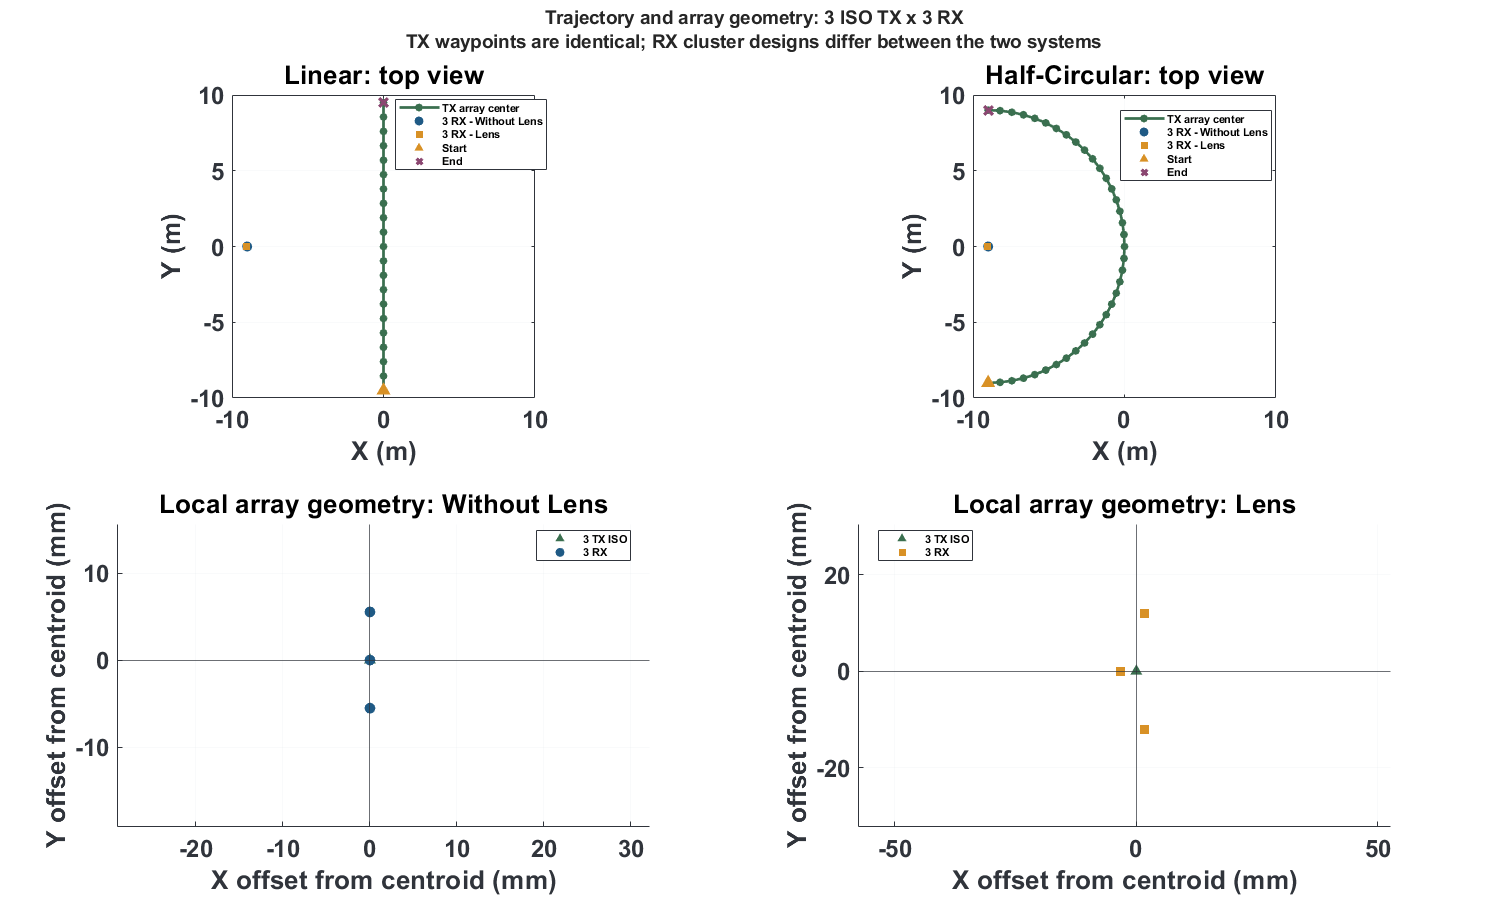
\includegraphics[width=\linewidth,height=4.05cm,keepaspectratio]
    {Analisis_v4_ISO_TX_Lens_vs_WithoutLens_Linear_HalfCircular_3x3/figures_matlab/01_geometry_and_arrays_matlab.png}
  \ThesisFigureCaption{3-1}{Matched TX trajectories and the two complete RX designs.}

  \column{0.38\textwidth}
  \scriptsize
  \begin{block}{Protocol A: placement comparison}
    Focal-arc lens RX versus linear baseline, both $3\times3$, at identical
    linear and half-circular waypoints.
  \end{block}
  \begin{block}{Protocol B: order comparison}
    Complete lens-assisted $3\times3$, $5\times5$, and $9\times9$ systems on one
    linear trajectory.
  \end{block}
  {\tiny\color{red!70!black}\textbf{Boundary:} placement and imported RX pattern
  change together.\par}
\end{columns}
\SourceNote{Chapter 3: Simulation Configuration and Paired Trajectories}
\note{
  \begin{itemize}
    \item In this section we test Antenna-lens-assisted MIMO communication performance.
    \item We will present the simulation configuration, the paired lens and baseline trajectories, and the evaluation metrics used to assess the system performance.
    \item We will also discuss the results of the paired lens and baseline trajectories, as well as the higher-order lens-assisted scaling.
  \end{itemize}
}
\end{frame}


\begin{frame}[t]{System-Level Simulation Configuration}
\scriptsize
\begin{columns}[T,onlytextwidth]
  \column{0.53\textwidth}
  \renewcommand{\arraystretch}{1.08}
  \begin{tabularx}{\linewidth}{@{}>{\bfseries}p{0.43\linewidth}X@{}}
    \toprule
    Parameter & Value\\
    \midrule
    Room / carrier & $20\times20\times3$~m / 38~GHz\\
    Bandwidth & 400~MHz, 401 bins\\
    TX array & 3 isotropic elements, 10~dBm each\\
    Mobility & 1~m/s; 16 time samples/waypoint\\
    Ray samples & 100{,}000 per source\\
    Linear path & 21 waypoints; 19.00~m\\
    Half-circle & 37 waypoints; 9~m radius\\
    \bottomrule
  \end{tabularx}

  \column{0.43\textwidth}
  \begin{block}{RX branch populations}
    Linear: $21\times3=63$ waypoint--RX observations per design.\par\smallskip
    Half-circle: $37\times3=111$ observations per design.
  \end{block}
  \begin{block}{Pattern contrast}
    Baseline branches reuse the $0^\circ$ patch pattern; lens branches use three
    angle-specific patterns at $+45^\circ$, $0^\circ$, and $-45^\circ$.
  \end{block}
  \MethodNote{Matching indices are ordinal design pairs, not co-located
  antenna elements.}
\end{columns}
\SourceNote{Chapter 3: Common Simulation Configuration}
\note{
  \begin{itemize}
    \item This parameter table shows the simulation configuration for the lens-assisted and baseline systems.
  \end{itemize}
}
\end{frame}


\begin{frame}[t]{Three Metric Scopes Answer Different Questions}
\scriptsize
\begin{columns}[T,onlytextwidth]
  \column{0.32\textwidth}
  \begin{block}{1. Link budget}
    \centering
    \begin{equation*}
      \begin{aligned}
        P_{\rm RX}&=P_{\rm TX}\sum_i|H_i|^2,\\[-1pt]
        C_{\rm link}&=\mathbb E_f[\log_2(1+\gamma)]
      \end{aligned}
      \tag{3.1}
    \end{equation*}
    \vspace{-0.4em}
    \raggedright
    Three simultaneous TX contributions feed one active RX branch. This retains
    absolute path loss and pattern gain.
  \end{block}

  \column{0.32\textwidth}
  \begin{block}{2. Constructed MIMO}
    \centering
    $\mathbf H_{N\times N}\leftarrow$ sequential $N\times1$ runs\par\smallskip
    \raggedright
    Condition number, effective rank, and equal-power capacity at a fixed
    normalized SNR of 10~dB diagnose channel structure.
  \end{block}

  \column{0.32\textwidth}
  \begin{block}{3. Spatial decorrelation}
    \centering
    \begin{equation*}
      D_{ij}=1-|\rho_{ij}|
      \tag{3.4}
    \end{equation*}
    \vspace{-0.4em}
    \raggedright
    Center-TX responses are evaluated by global pooling, waypoint-local
    pooling, and block-median statistics.
  \end{block}
\end{columns}
\CautionNote{These metrics have different normalization and weighting. In
particular, $C_{\rm link}$ and fixed-10-dB constructed-MIMO capacity are not
numerically interchangeable.}
\SourceNote{Chapter 3: Evaluation Metrics and Aggregation}
\note{
  \begin{itemize}
    \item There are 3 metric scopes to answer different questions: link budget, constructed MIMO, and spatial decorrelation.
    \item For the constructed-MIMO scope, each sequential $N\times1$ channel
    realization forms one column of
    $\mathbf H(f)=[\mathbf h_1(f)\ \mathbf h_2(f)\ \cdots\ \mathbf h_N(f)]$,
    producing a constructed $N\times N$ channel matrix.
    \item From its singular values, the condition number and effective rank are
    $\kappa(f)=\sigma_1(f)/\sigma_3(f)$ and
    $r_{\mathrm{eff}}(f)=\exp[-\sum_{i=1}^{3}p_i(f)\ln p_i(f)]$, where
    $p_i(f)=\sigma_i^2(f)/\sum_{j=1}^{3}\sigma_j^2(f)$, as given in
    Equation~(3.2).
    \item The equal-power constructed-MIMO capacity is
    $C_{\mathrm{MIMO}}(\gamma)=\mathbb E_f[\sum_{i=1}^{3}
    \log_2(1+\gamma\sigma_i^2(f)/N_t)]$, with $N_t=3$, as given in
    Equation~(3.3).
    \item Emphasize that the matrix combines sequential simulations and is used
    to diagnose channel structure and diversity potential; it is not a directly
    measured simultaneous three-port channel.
  \end{itemize}
}
\end{frame}


\begin{frame}[t]{A Static Snapshot Shows Gain --- but Mixed MIMO Structure}
\begin{columns}[T,onlytextwidth]
  \column{0.59\textwidth}
  \centering
  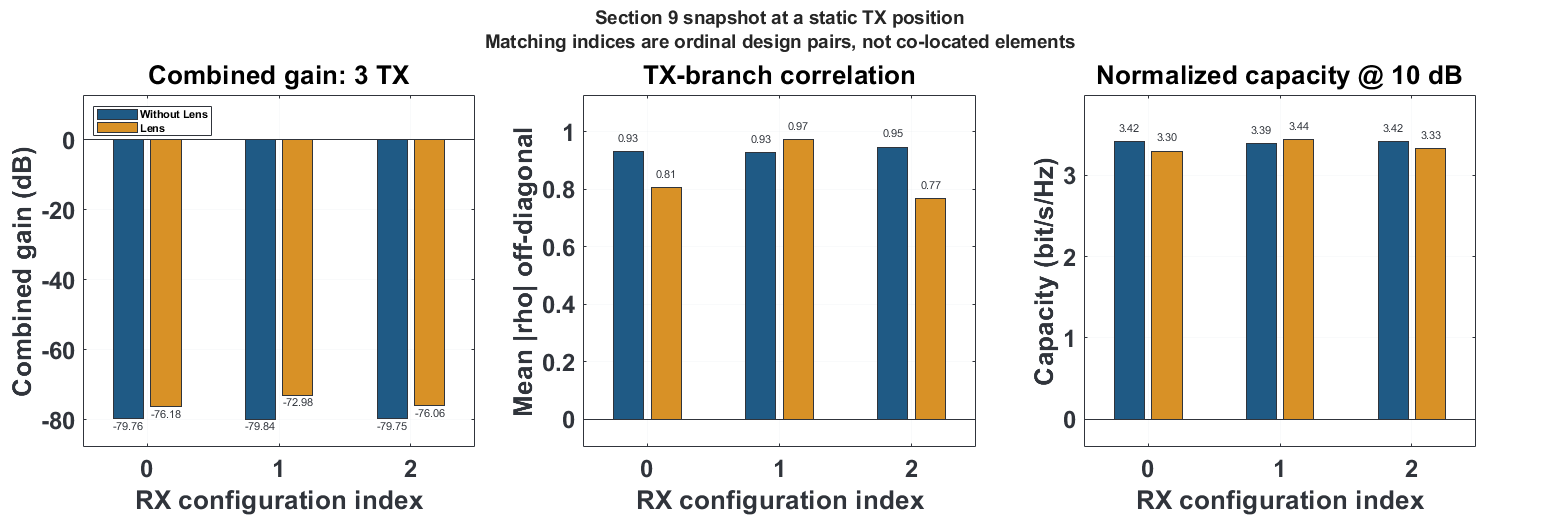
\includegraphics[width=\linewidth,height=4.95cm,keepaspectratio]
    {Analisis_v4_ISO_TX_Lens_vs_WithoutLens_Linear_HalfCircular_3x3/figures_matlab/02_static_rx_scenario_comparison_matlab.png}
  \ThesisFigureCaption{3-2}{Static branch gain, TX correlation, and normalized capacity.}

  \column{0.37\textwidth}
  \scriptsize
  \begin{block}{Absolute branch gain}
    Lens branches span $-76.18$ to $-72.98$~dB; baseline spans only
    $-79.84$ to $-79.75$~dB.
  \end{block}
  \begin{block}{Constructed $3\times3$ snapshot}
    \renewcommand{\arraystretch}{1.12}
    \begin{tabular}{@{}lcc@{}}
      & Base & Lens\\\midrule
      $\kappa$ (dB) & \textbf{23.90} & 28.70\\
      $r_{\rm eff}$ & 1.42 & \textbf{1.60}\\
      $C_{\rm MIMO}$ & 6.81 & \textbf{7.24}\\
      RX corr. & 0.7927 & \textbf{0.5636}
    \end{tabular}
  \end{block}
  % \CautionNote{A better condition number alone does not prove stronger
  % multiplexing.}
\end{columns}
\SourceNote{Chapter 3: Static Snapshot Characterization}
\note{
  \begin{itemize}
    \item This snapshot shows the performance of the lens-assisted and baseline systems at a static point in time.
    \item The lens has better absolute branch gain, but the constructed MIMO metrics show mixed results.
    \item The lens improves rank, normalized capacity, and RX correlation in this snapshot, while its condition number becomes worse.
    \item This is a normalized single-position result. It does not imply that
          every lens branch retains a gain or capacity advantage as the TX moves
          along either trajectory.
  \end{itemize}
}
\end{frame}


\begin{frame}[t]{Equal-Weight Trajectory Aggregation Favors the Baseline}
\scriptsize
\centering
\renewcommand{\arraystretch}{1.18}
\begin{tabular}{@{}llrrrrrr@{}}
  \toprule
  Path & RX & $|H|_{\rm med}$ & $C_{\rm link}$ & $\kappa$ & $r_{\rm eff}$ & $C_{\rm MIMO}$ & $D_{\rm med}$\\
  \midrule
  Linear & Base & $-79.74$ & \textbf{5.41} & \textbf{25.01} & \textbf{1.202} & \textbf{6.12} & 0.0909\\
  Linear & Lens & $-86.75$ & 3.57 & 25.55 & 1.154 & 5.85 & \textbf{0.5308}\\
  Half-circle & Base & $-80.89$ & \textbf{5.08} & 25.58 & \textbf{1.348} & \textbf{6.71} & 0.0638\\
  Half-circle & Lens & $-87.29$ & 3.53 & \textbf{21.56} & 1.305 & 6.58 & \textbf{0.5518}\\
  \bottomrule
\end{tabular}

\vspace{0.35cm}
\begin{columns}[T,onlytextwidth]
  \column{0.48\textwidth}
  \MethodNote{\textbf{Aggregate rate and rank:} all three directional RX cases
  receive equal statistical weight, including persistently misaligned beams.}
  \column{0.48\textwidth}
  \MethodNote{\textbf{Local angular differentiation:} block-median
  decorrelation strongly favors the lens on both paths.}
\end{columns}
% \Takeaway{The lens improves selectivity, but equal weighting does not convert
% that selectivity into higher aggregate capacity.}
\SourceNote{Chapter 3: Aggregate Placement-Comparison Results; capacities in bit/s/Hz}
\note{
  \fontsize{7}{8}\selectfont
  \begin{itemize}
    \setlength{\itemsep}{0.3em}
    \setlength{\parskip}{0pt}
    \item This table compares the lens-assisted and baseline RX systems along
          the linear and half-circular trajectories.
    \item Equal-weight aggregation gives the same statistical weight to all
          three directional RX branches, including weak or misaligned lens
          branches; no beam selection is applied.
    \item Under this rule, the baseline achieves higher link capacity,
          effective rank, and MIMO capacity on both trajectories. This result is
          consistent with its more uniform branch response as the transmitter
          moves; it does not isolate antenna pattern from RX placement.
    \item The lens nevertheless provides much stronger median-block
          decorrelation, confirming useful local angular selectivity.
    \item Therefore, the lens is not universally worse. Its selectivity must be
          exploited through beam selection or adaptive combining to avoid
          persistently misaligned branches and potentially improve capacity.
    \item The takeaway is that the lens improves selectivity, but equal weighting does not convert that selectivity into higher aggregate capacity.
  \end{itemize}
}
\end{frame}


\begin{frame}[t]{Along Both Paths, Branch Alignment Drives a Wide Lens Spread}
\centering
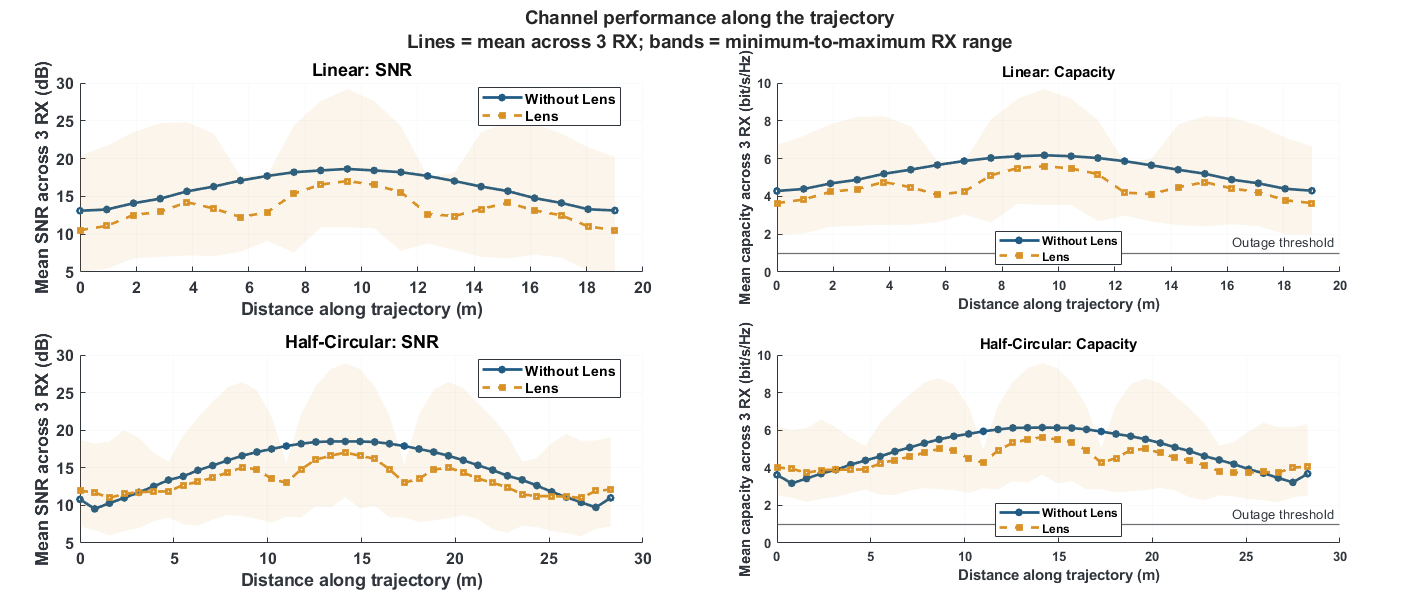
\includegraphics[width=0.92\linewidth,height=4.55cm,keepaspectratio]
  {Analisis_v4_ISO_TX_Lens_vs_WithoutLens_Linear_HalfCircular_3x3/figures_matlab/04_channel_metrics_along_trajectory_matlab.png}
\ThesisFigureCaption{3-5}{Mean SNR and equivalent-SISO capacity; shaded lens
bands are RX-branch minima--maxima.}
\begin{columns}[T,onlytextwidth]
  \column{0.48\textwidth}
  \MethodNote{The baseline mean is higher at all 21 linear waypoints and at 28
  of 37 half-circle waypoints; aligned lens branches reverse the mean locally.}
  \column{0.48\textwidth}
  \CautionNote{All cases have 0\% outage at 1~bit/s/Hz; this threshold is
  saturated and cannot distinguish reliability.}
\end{columns}
\note{
  \fontsize{7}{8}\selectfont
  \begin{itemize}
    \setlength{\itemsep}{0.3em}
    \setlength{\parskip}{0pt}
    \item The solid and dashed lines are means across the three RX design
          cases. The shaded lens region is the minimum-to-maximum branch range,
          not a confidence interval.
    \item On the linear path, the baseline mean capacity is higher at all 21
          waypoints. On the half-circle, it is higher at 28 of 37 waypoints.
    \item The remaining half-circle positions show that a locally aligned lens
          branch can raise the three-branch mean above the baseline. The lens is
          therefore not weaker at every position, even though its aggregate
          median is lower.
    \item The much wider lens band is evidence of angular selectivity: one
          branch may align strongly while another remains weak at the same
          waypoint.
    \item Every configuration records 0\% outage at 1~bit/s/Hz. This threshold
          is saturated, so it cannot support a reliability comparison; a higher
          threshold or capacity percentiles would be more informative.
  \end{itemize}
}
\end{frame}


\begin{frame}[t]{The Constructed MIMO Channel Has a Geometry Bottleneck}
\centering
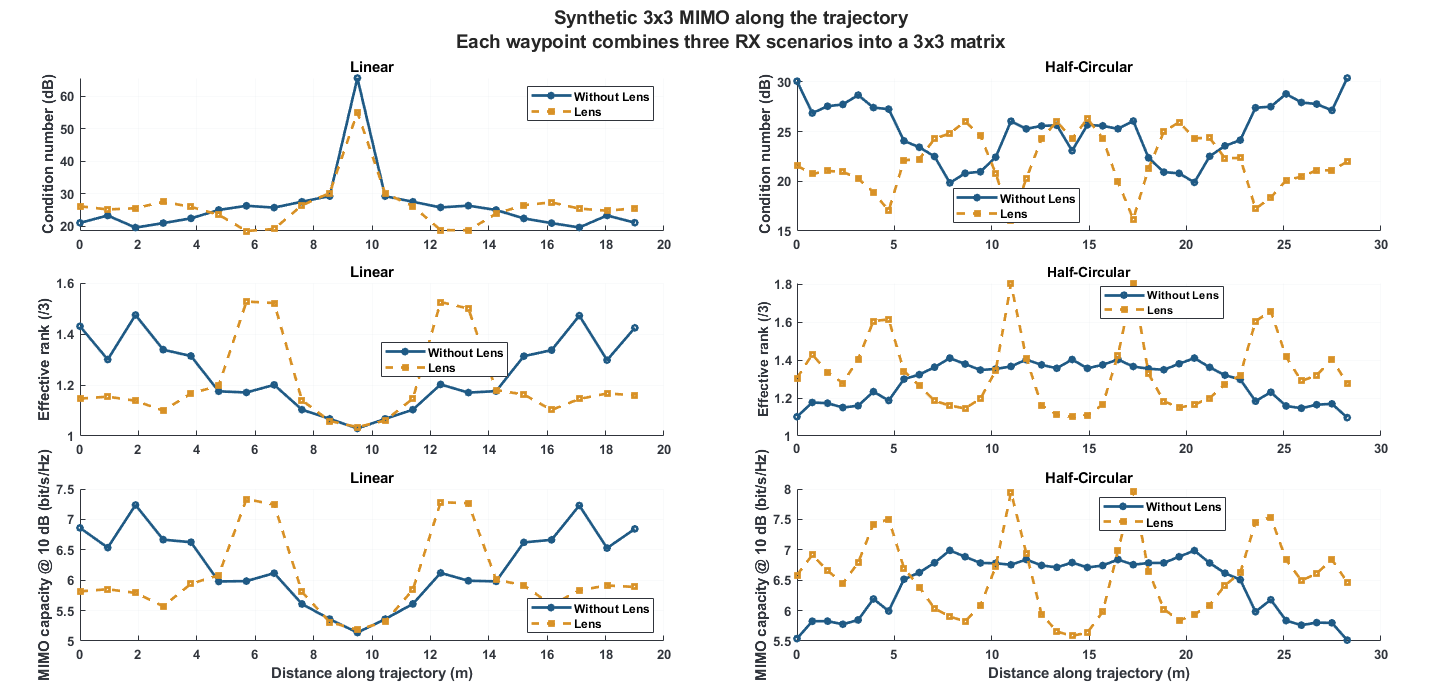
\includegraphics[width=0.91\linewidth,height=4.35cm,keepaspectratio]
  {Analisis_v4_ISO_TX_Lens_vs_WithoutLens_Linear_HalfCircular_3x3/figures_matlab/05_trajectory_mimo_metrics_matlab.png}
\ThesisFigureCaption{3-6}{Conditioning, effective rank, and fixed-10-dB
constructed-MIMO capacity.}
\begin{columns}[T,onlytextwidth]
  \column{0.48\textwidth}
  \MethodNote{At the 9.5~m linear midpoint, $\kappa$ reaches 65.69~dB
  (baseline) and 55.09~dB (lens).}
  \column{0.48\textwidth}
  \MethodNote{The half-circle avoids this isolated symmetry-related impairment
  and gives higher median rank and capacity for both designs.}
\end{columns}
\SourceNote{Chapter 3: Constructed MIMO Performance Along the Trajectories}
\note{
  \fontsize{7}{8}\selectfont
  \begin{itemize}
    \setlength{\itemsep}{0.3em}
    \setlength{\parskip}{0pt}
    \item This figure compares the constructed-MIMO conditioning, effective
          rank, and fixed-10-dB capacity along both trajectories.
    \item Under the evaluated equal-weight configuration, the lens generally
          has lower effective rank and MIMO capacity than the baseline. Its
          angular selectivity does not become a multiplexing gain when weak or
          misaligned branches remain included.
    \item The condition-number result is mixed: the lens is 0.55~dB worse in
          median on the linear path but 4.02~dB better on the half-circle.
    \item At the 9.5~m linear midpoint, geometric symmetry creates an isolated
          bottleneck. The condition number reaches 65.69~dB for the baseline
          and 55.09~dB for the lens. The lens reduces the severity, but both
          channels remain extremely ill-conditioned.
    \item The half-circle avoids this symmetry-related impairment and gives
          higher median rank and capacity for both designs, showing that
          deployment geometry remains a dominant factor.
    \item Therefore, the lens is not worse for every metric, but it
          underperforms the baseline in the main multiplexing metrics under
          this operating rule. Beam selection or adaptive combining is needed
          to exploit its directional response.
  \end{itemize}
}
\end{frame}


\begin{frame}[t]{Lens Decorrelation Gain Depends on Aggregation Scope}
\begin{columns}[T,onlytextwidth]
  \column{0.61\textwidth}
  \centering
  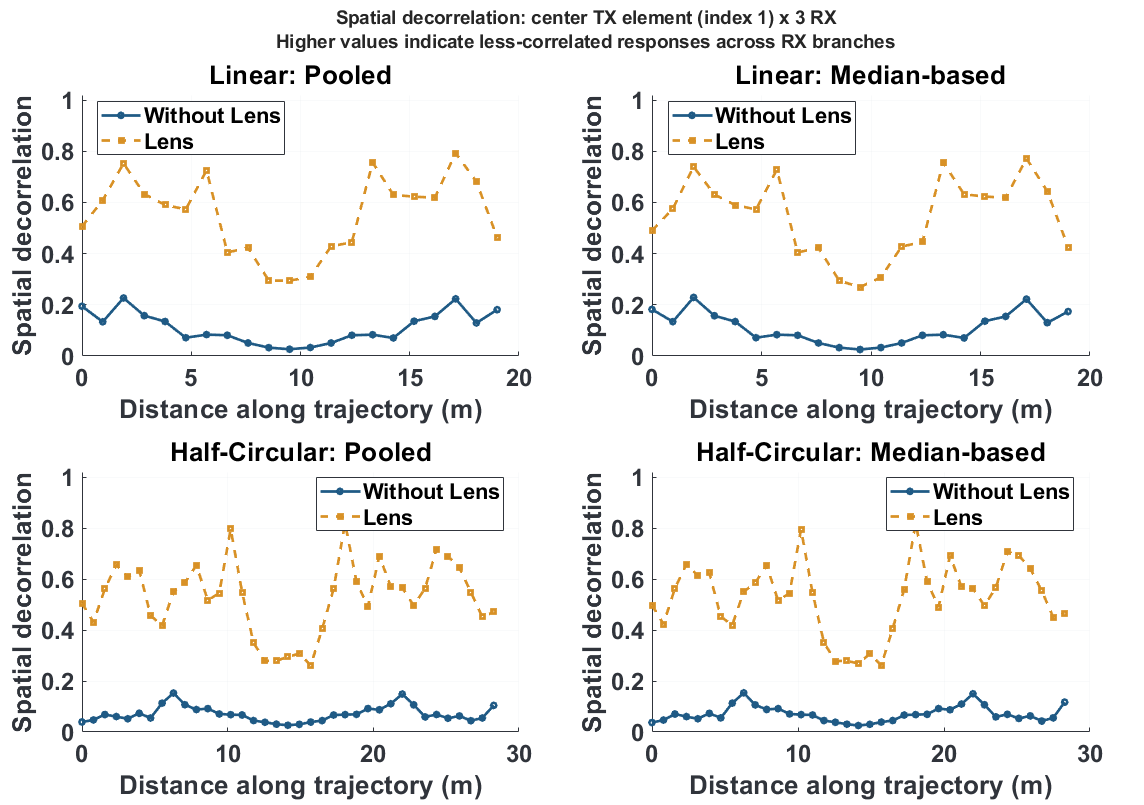
\includegraphics[width=\linewidth,height=4.35cm,keepaspectratio]
    {Analisis_v4_ISO_TX_Lens_vs_WithoutLens_Linear_HalfCircular_3x3/figures_matlab/06_spatial_decorrelation_comparison_matlab.png}
  \ThesisFigureCaption{3-7}{Waypoint-local decorrelation of the center-TX response.}

  \column{0.35\textwidth}
  \scriptsize
  \begin{block}{Global pooled}
    Lens rises only slightly: 0.9784 to 0.9807 (linear) and 0.9744 to 0.9872
    (half-circle).
  \end{block}
  \begin{block}{Typical local block}
    Lens $D_{\rm med}$: 0.5308 / 0.5518.\par
    Baseline: 0.0909 / 0.0638.
  \end{block}
  {\tiny\color{red!70!black}\textbf{Not equivalent to} the singular-value
  structure of the constructed $3\times3$ matrix.\par}
\end{columns}
% \Takeaway{Both estimators favor the lens; aggregation scope determines whether
% the measured increase is slight or substantial.}
\SourceNote{Chapter 3: Spatial Decorrelation}
\note{
  \fontsize{7}{8}\selectfont
  \begin{itemize}
    \setlength{\itemsep}{0.3em}
    \setlength{\parskip}{0pt}
    \item This slide shows that the decorrelation result depends on the
          aggregation scope and on where normalization is applied. A higher
          $D=1-|\rho|$ means less-correlated RX responses.
    \item Global pooling concatenates all waypoint, time, and frequency samples
          before computing correlation. Under this estimator the lens is only
          slightly higher on both trajectories.
    \item The block-median estimator evaluates correlation locally before
          taking a typical value. It strongly favors the lens: $D_{\rm med}$
          increases from 0.0909 to 0.5308 on the linear path and from 0.0638 to
          0.5518 on the half-circle.
    \item The effect sizes differ because global pooling measures the coherence
          of the complete concatenated trajectory, whereas the local estimator
          shows that a typical lens block has more differentiated
          angle-dependent responses.
    \item Thus, aggregation changes the magnitude of the observed lens benefit,
          not its direction: both global-pooled and block-median decorrelation
          are higher with the lens in this $3\times3$ comparison.
    \item This calculation uses only the center-TX response across three RX
          branches. It is not equivalent to the singular values, effective
          rank, or multiplexing performance of the constructed $3\times3$
          MIMO matrix.
    \item The appropriate conclusion is that the lens provides stronger local
          angular selectivity, not that it automatically provides higher MIMO
          capacity.
    \item Takeaway: both estimators favor the lens; aggregation scope determines whether the measured increase is slight or substantial.
  \end{itemize}
}
\end{frame}


\begin{frame}[t]{System-Level Interpretation: Select, Combine, or Pay the Penalty}
\centering
\resizebox{0.92\linewidth}{!}{%
\begin{tikzpicture}[>=latex,font=\footnotesize,node distance=0.70cm]
  \node[draw=Blue,fill=SoftBlue,rounded corners,minimum width=3.3cm,
        minimum height=1.0cm,align=center] (lens) {lens produces\\angle-specific branches};
  \node[draw=Teal,fill=SoftTeal,rounded corners,minimum width=3.3cm,
        minimum height=1.0cm,align=center,right=1.2cm of lens] (spread) {large within-waypoint\\capacity spread};
  \node[draw=Gold!85!black,fill=SoftGold,rounded corners,minimum width=3.3cm,
        minimum height=1.0cm,align=center,right=1.2cm of spread] (decision) {receiver operating rule};
  \node[draw=red!70!black,rounded corners,minimum width=4.0cm,
        minimum height=1.0cm,align=center,below left=1.25cm and -0.1cm of decision] (equal) {equal weighting\\misaligned branches reduce aggregate rate};
  \node[draw=Teal,rounded corners,minimum width=4.0cm,
        minimum height=1.0cm,align=center,below right=1.25cm and -0.1cm of decision] (adapt) {beam selection / combining\\can exploit the strongest local branch};
  \draw[->,thick] (lens)--(spread);
  \draw[->,thick] (spread)--(decision);
  \draw[->,thick] (decision)--(equal);
  \draw[->,thick] (decision)--(adapt);
\end{tikzpicture}}

\vspace{0.45cm}
\begin{columns}[T,onlytextwidth]
  \column{0.48\textwidth}
  \CautionNote{Measured result in this thesis: equal-weight lens aggregation
  yields lower median link and constructed-MIMO capacity.}
  \column{0.48\textwidth}
  \MethodNote{Design implication: the lens is an angularly selective front end,
  not a uniform-gain replacement for a coplanar array.}
\end{columns}
\SourceNote{Chapter 3: Discussion and Placement-Comparison Summary}
\note{
  \fontsize{7}{8}\selectfont
  \begin{itemize}
    \setlength{\itemsep}{0.3em}
    \setlength{\parskip}{0pt}
    \item The system-level conclusion is that the lens behaves as an
          angle-selective front end, rather than as a uniform-gain replacement
          for a conventional coplanar array.
    \item Its directional branches produce a wide capacity spread at each
          waypoint: an aligned branch can be strong, while misaligned branches
          can remain weak.
    \item The receiver operating rule therefore determines whether this
          selectivity becomes useful. Giving every branch equal weight retains
          the weak branches and reduces the aggregate link and constructed-MIMO
          capacity in the results of this thesis.
    \item Beam selection or adaptive combining could instead emphasize the
          strongest locally aligned branch and avoid persistently misaligned
          responses.
    \item However, this adaptive strategy is a design implication and future
          research direction; it was not directly evaluated in the present
          equal-weight simulations.
    \item The appropriate conclusion is not that the lens is universally
          better or worse, but that its benefit is conditional on alignment
          and on how the receiver processes the angle-specific branches.
  \end{itemize}
}
\end{frame}


\subsection{Higher-Order Lens-Assisted Scaling}

\begin{frame}[t]{Higher-Order Study Changes Power, Aperture, and Angular Grid}
\begin{columns}[T,onlytextwidth]
  \column{0.61\textwidth}
  \centering
  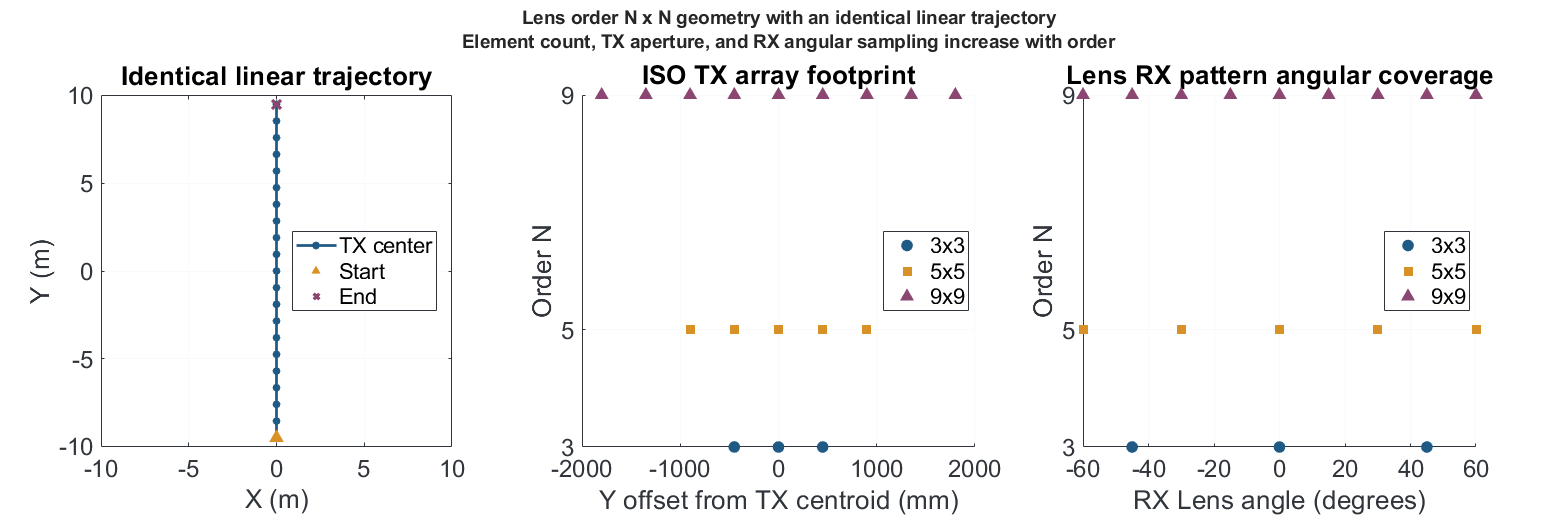
\includegraphics[width=\linewidth,height=4.50cm,keepaspectratio]
    {Analisis_v4_ISO_TX_Lens_Order_3x3_5x5_9x9_Linear/figures_matlab/01_geometry_order_comparison_matlab.png}
  \ThesisFigureCaption{3-9}{Common linear path with order-dependent TX and RX geometry.}

  \column{0.35\textwidth}
  \scriptsize
  \setlength{\tabcolsep}{2pt}
  \renewcommand{\arraystretch}{1.10}
  \begin{tabular}{@{}lrrr@{}}
    \toprule
    $N$ & Aperture & RX step & $P_{\rm TX,tot}$\\
    \midrule
    3 & 0.90~m & $45^\circ$ & 14.77~dBm\\
    5 & 1.80~m & $30^\circ$ & 16.99~dBm\\
    9 & 3.60~m & $15^\circ$ & 19.54~dBm\\
    \bottomrule
  \end{tabular}

  \vspace{0.30cm}
  \begin{block}{Normalization}
    \[
      \eta_r=\frac{r_{\rm eff}}{N},\qquad
      \eta_C=\frac{C_{\rm MIMO}}{N}
    \]
  \end{block}
  \CautionNote{This is complete-design scaling, not a causal test of order $N$
  alone.}
\end{columns}
\SourceNote{Chapter 3: Higher-Order Simulation Configuration}
\end{frame}


\begin{frame}[t]{Higher Order Raises Capacity but Lowers Efficiency}
\scriptsize
\begin{columns}[T,onlytextwidth]
  \column{0.47\textwidth}
  \renewcommand{\arraystretch}{1.18}
  \begin{tabularx}{\linewidth}{@{}Xrrr@{}}
    \toprule
    Metric & $3\times3$ & $5\times5$ & $9\times9$\\
    \midrule
    $C_{\rm link}$ & 3.57 & 4.13 & \textbf{5.19}\\
    $\kappa$ (dB) & \textbf{25.55} & 34.24 & 42.88\\
    $r_{\rm eff}$ & 1.154 & 1.332 & \textbf{2.043}\\
    $\eta_r$ & \textbf{0.385} & 0.266 & 0.227\\
    $C_{\rm MIMO}$ & 5.851 & 8.254 & \textbf{14.562}\\
    $\eta_C$ & \textbf{1.950} & 1.651 & 1.618\\
    $D_{\rm global}$ & \textbf{0.9807} & 0.9276 & 0.8570\\
    $D_{\rm med}$ & \textbf{0.5308} & 0.5166 & 0.4876\\
    \bottomrule
  \end{tabularx}
  \SlideCaption{Trajectory medians; capacities in bit/s/Hz}

  \column{0.49\textwidth}
  \centering
  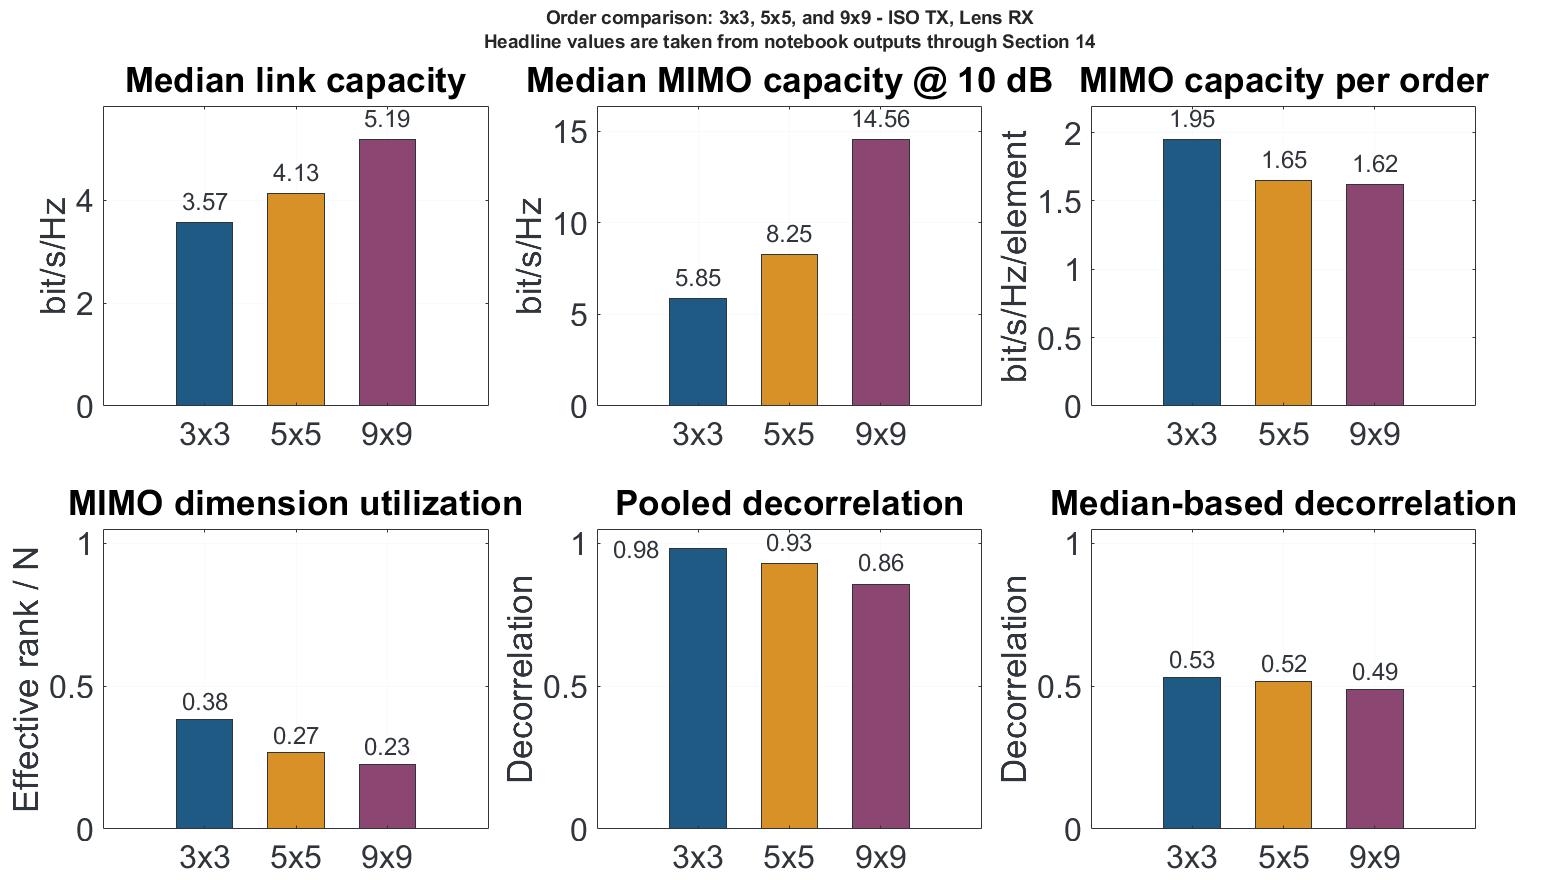
\includegraphics[width=\linewidth,height=4.85cm,keepaspectratio]
    {Analisis_v4_ISO_TX_Lens_Order_3x3_5x5_9x9_Linear/figures_matlab/08_aggregate_order_comparison_matlab.png}
  \ThesisFigureCaption{3-12}{Absolute, normalized, and decorrelation metrics.}
\end{columns}
% \Takeaway{$3\times3\rightarrow9\times9$: fixed-10-dB capacity rises 148.9\%,
% but rank fraction falls 41.0\% and capacity per dimension falls 17.0\%.}
\SourceNote{Chapter 3: Aggregate Higher-Order Results}
\note{
  \fontsize{7}{8}\selectfont
  \begin{itemize}
    \setlength{\itemsep}{0.3em}
    \setlength{\parskip}{0pt}
    \item This slide separates the benefit of adding dimensions from the
          efficiency with which those dimensions are used.
    \item From $3\times3$ to $9\times9$, link capacity rises from 3.57 to
          5.19~bit/s/Hz, and fixed-10-dB constructed-MIMO capacity rises by
          148.9\%, from 5.851 to 14.562~bit/s/Hz.
    \item However, conditioning worsens as $\kappa$ increases from 25.55 to
          42.88~dB. Although absolute effective rank increases, the rank
          fraction $\eta_r$ falls by 41.0\%, showing that a smaller fraction of
          the available dimensions remains effective.
    \item Capacity per dimension $\eta_C$ also falls by 17.0\%, and both
          decorrelation estimators decrease. The additional dimensions are
          therefore increasingly correlated and less efficiently utilized.
    \item The conclusion is that higher order increases total capacity, but
          with diminishing spatial efficiency. This is complete-design scaling,
          not an order-only effect, because transmit power, aperture, and the
          angular grid also change with $N$.
    \item Takeaway : {$3\times3\rightarrow9\times9$: fixed-10-dB capacity rises 148.9\%,
but rank fraction falls 41.0\% and capacity per dimension falls 17.0\%.}
  \end{itemize}
}
\end{frame}


\begin{frame}[t]{More Dimensions Do Not Remove Geometry-Limited Modes}
\begin{columns}[T,onlytextwidth]
  \column{0.62\textwidth}
  \centering
  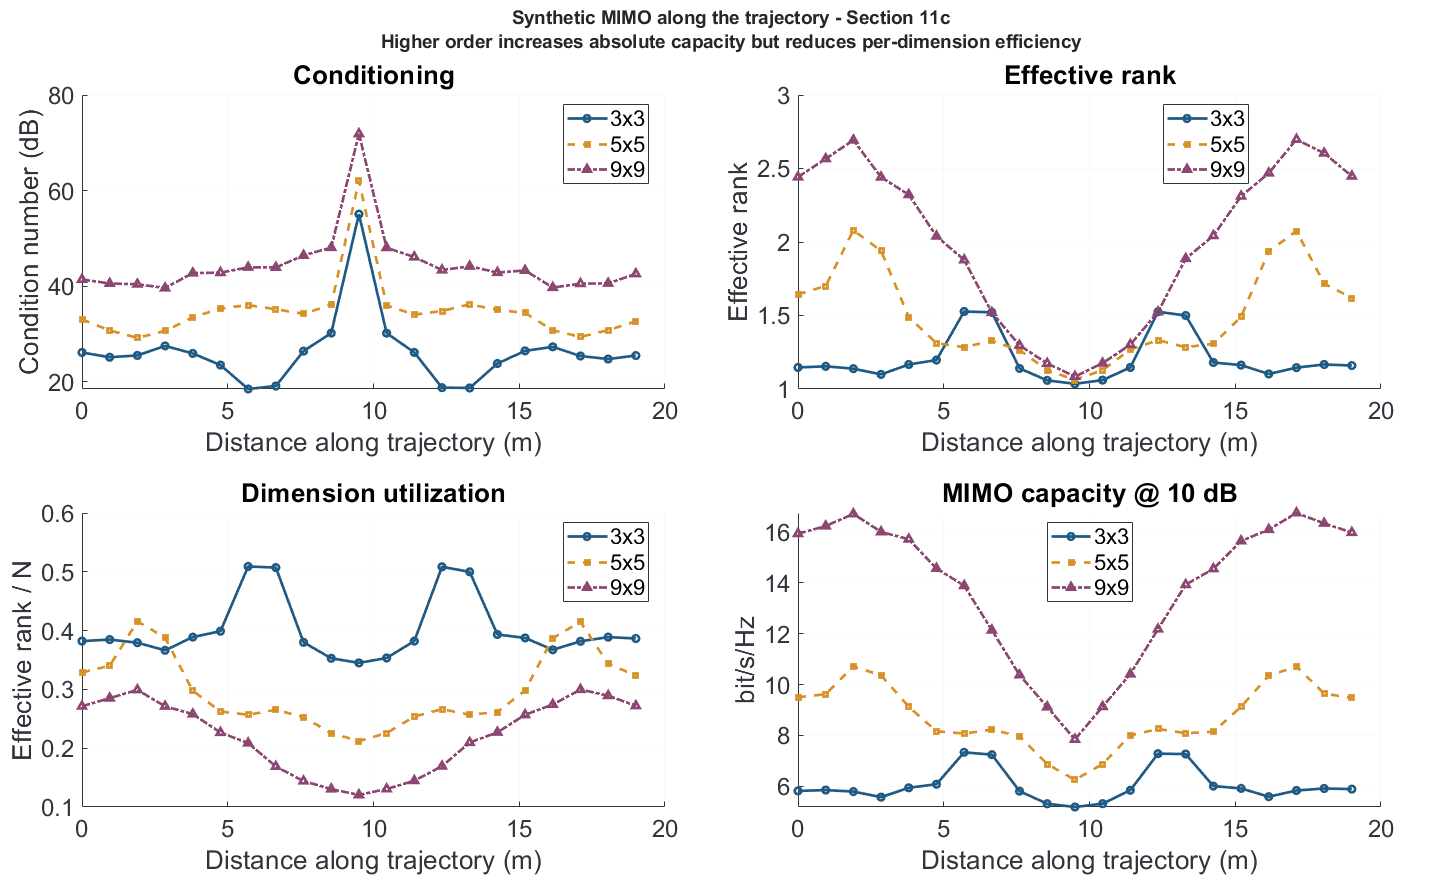
\includegraphics[width=\linewidth,height=4.05cm,keepaspectratio]
    {Analisis_v4_ISO_TX_Lens_Order_3x3_5x5_9x9_Linear/figures_matlab/05_trajectory_mimo_scaling_matlab.png}
  \ThesisFigureCaption{3-14}{Order-dependent conditioning, rank efficiency, and capacity.}

  \column{0.34\textwidth}
  \scriptsize
  \begin{block}{Shared midpoint bottleneck}
    At 9.5~m, $r_{\rm eff}\approx1$ for every order; $\kappa$ worsens from
    55.09 to 71.89~dB.
  \end{block}
  \begin{block}{Decorrelation trend}
    Global and block-median decorrelation decrease as the RX pair population
    grows and angular spacing tightens.
  \end{block}
  {\tiny\color{red!70!black}\textbf{Confounds:} +4.77~dB total TX power,
  fourfold aperture, and only one common RX angle.\par}
\end{columns}

\SourceNote{Chapter 3: Constructed MIMO Scaling and Spatial Decorrelation}
\note{
  \fontsize{7}{8}\selectfont
  \begin{itemize}
    \setlength{\itemsep}{0.3em}
    \setlength{\parskip}{0pt}
    \item This figure shows that adding more antenna dimensions does not remove
          a geometry-induced channel bottleneck.
    \item At the 9.5~m midpoint, the effective rank collapses to approximately
          one for every order. The condition number also worsens from 55.09~dB
          for $3\times3$ to 71.89~dB for $9\times9$.
    \item Thus, when the propagation geometry makes the channel responses
          nearly dependent, a larger array adds nominal dimensions but does not
          create an equal number of usable spatial modes.
    \item Global and block-median decorrelation decrease with order, consistent
          with greater similarity among the growing RX-pair population and the
          tighter angular spacing.
    \item This trend cannot be attributed to $N$ alone: total TX power rises by
          4.77~dB, the aperture changes by a factor of four, and the compared
          angular grids share only one common RX angle.
    \item The safe conclusion is that higher order raises absolute capacity,
          but geometry-limited modes remain and spatial efficiency decreases.
    \item Takeaway : Higher order adds capacity, but its dimensions are less balanced and
less efficiently utilized.
  \end{itemize}
}
\end{frame}

% !TEX root = ../BeamerTemplate.tex
%%%%%%%%%%%%%%%%%%%%%%%%%%%%%%%%%%%%%%%%%%%%%%%%%%%%%%%%%%%%%%%%%%%%%%%%%%%%%%%%%%

\section{Conclusions and Future Work}

\begin{frame}[t]{The Four Research Questions Receive Conditional Answers}
\scriptsize
\begin{columns}[T,onlytextwidth]
  \column{0.49\textwidth}
  \begin{block}{RQ1 --- Physical realization: supported}
    The $20\times20$ transmitarray produces a realized focus near 14~mm, a
    focal arc, and angle-dependent far-field responses.
  \end{block}
  \begin{block}{RQ3 --- Mobile comparison: no universal gain}
    Under equal weighting, the baseline has higher median link and constructed
    MIMO capacity; the lens has stronger typical-block decorrelation.
  \end{block}

  \column{0.49\textwidth}
  \begin{block}{RQ2 --- Cross-solver trend: mostly supported}
    All solvers predict matched-link reinforcement, cross-link suppression,
    lower correlation, and higher raw capacity; normalized gains differ.
  \end{block}
  \begin{block}{RQ4 --- Higher order: gain with lower efficiency}
    Capacity grows from $3\times3$ to $9\times9$, while conditioning, rank
    fraction, and capacity per dimension deteriorate.
  \end{block}
\end{columns}
\Takeaway{The spatial transformation is real; its system benefit depends on
receiver operation and geometry.}
\SourceNote{Chapter 4: Principal Findings}
\end{frame}


\begin{frame}[t]{Principal Contributions}
\scriptsize
\begin{columns}[T,onlytextwidth]
  \column{0.49\textwidth}
  \begin{block}{Physical and computational bridge}
    \raggedright
    \begin{itemize}
      \setlength{\itemsep}{0.30em}
      \item Full-wave characterized planar $20\times20$ transmitarray and
            focal-plane RX arrangement at 38~GHz.
      \item Common raw/normalized MIMO framework for HFSS S-parameters and
            Sionna-RT channel responses.
      \item Three-solver evidence with 92.6\% agreement on the sign of the
            link-level lens effect.
    \end{itemize}
  \end{block}

  \column{0.49\textwidth}
  \begin{block}{System-level evidence}
    \raggedright
    \begin{itemize}
      \setlength{\itemsep}{0.30em}
      \item Paired mobile study explaining why local decorrelation does not
            automatically increase aggregate capacity.
      \item Explicit comparison of global, waypoint-local, and block-median
            decorrelation estimators.
      \item Higher-order evidence of absolute capacity growth with declining
            per-dimension efficiency.
    \end{itemize}
  \end{block}
\end{columns}
\SourceNote{Chapter 4: Contributions}
\end{frame}


\begin{frame}[t]{Overall Conclusion: Focusing Is Necessary but Not Sufficient}
\small
\begin{columns}[T,onlytextwidth]
  \column{0.31\textwidth}
  \begin{block}{What works}
    Passive focusing and angular filtering reshape channel amplitudes and
    improve local separability.
  \end{block}
  \column{0.31\textwidth}
  \begin{block}{What limits it}
    Misalignment, equal branch weighting, and geometry-limited singular modes
    can erase the link-level benefit.
  \end{block}
  \column{0.31\textwidth}
  \begin{block}{What is required}
    Placement, channel geometry, normalization, and beam management must be
    designed jointly.
  \end{block}
\end{columns}

\vspace{0.35cm}
\begin{beamercolorbox}[rounded=true,sep=1.0ex,wd=\linewidth]{takeaway}
  \centering\large\bfseries
  The transmitarray is an effective passive spatial transformer --- not an
  automatic MIMO-capacity multiplier.
\end{beamercolorbox}
\SourceNote{Chapter 4: Overall Conclusion}
\end{frame}


\begin{frame}[t]{Limitations I: Physical Validation and Channel Construction}
\scriptsize
\begin{columns}[T,onlytextwidth]
  \column{0.49\textwidth}
  \begin{block}{Physical and numerical validation}
    \begin{itemize}
      \setlength{\itemsep}{0.15em}
      \item Simulation only; no fabricated prototype or coherent OTA channel.
      \item Solver formulations and absolute reference quantities differ.
      \item Realized 14~mm focus differs from the 30~mm design target.
    \end{itemize}
  \end{block}

  \column{0.49\textwidth}
  \begin{block}{Receiver construction}
    \begin{itemize}
      \setlength{\itemsep}{0.15em}
      \item $N\times N$ matrices stack sequential $N\times1$ simulations.
      \item Mutual coupling, common phase, switching overhead, and joint RX
            noise are omitted.
      \item The reconstructed matrix is a controlled proxy, not a simultaneous
            measured multiport channel.
    \end{itemize}
  \end{block}
\end{columns}
\CautionNote{Absolute values from different solvers and channel constructions
are not directly interchangeable.}
\SourceNote{Chapter 4: Limitations}
\end{frame}


\begin{frame}[t]{Limitations II: Fair Comparison and Reproducibility}
\scriptsize
\begin{columns}[T,onlytextwidth]
  \column{0.49\textwidth}
  \begin{block}{Comparison confounds}
    \begin{itemize}
      \setlength{\itemsep}{0.15em}
      \item Lens and baseline designs differ in both placement and pattern.
      \item Order study changes power, aperture, RX count, and angular grid.
      \item Only the $0^\circ$ receive branch is common across all array orders.
    \end{itemize}
  \end{block}

  \column{0.49\textwidth}
  \begin{block}{Sampling and reproducibility}
    \begin{itemize}
      \setlength{\itemsep}{0.15em}
      \item One room and controlled trajectories; no multi-seed confidence
            intervals or convergence sweep.
      \item 100{,}000 ray samples/source; outage is saturated.
      \item Source notebooks and complete complex tensors are absent from the
            current trajectory archive.
    \end{itemize}
  \end{block}
\end{columns}
\CautionNote{Evidence supports controlled mechanisms, not universal deployment
performance.}
\SourceNote{Chapter 4: Limitations}
\end{frame}


\begin{frame}[t]{Future Work: Turn Angular Selectivity into Operational Gain}
\scriptsize
\begin{columns}[T,onlytextwidth]
  \column{0.49\textwidth}
  \begin{block}{1. Measure the physical system}
    Fabricate the feed and transmitarray; measure focal distance, patterns, and
    simultaneous coherent multiport channels.
  \end{block}
  \begin{block}{3. Make comparisons causal and fair}
    Isolate placement from pattern, then hold total TX power, aperture, and RX
    angle set fixed across orders.
  \end{block}

  \column{0.49\textwidth}
  \begin{block}{2. Add adaptive beam management}
    Evaluate selection, switching, combining, and hybrid beamforming with
    training overhead and alignment error.
  \end{block}
  \begin{block}{4. Broaden and reproduce the evidence}
    Retain tensors and notebooks; add seeds, convergence tests, blockage,
    mobility, richer scenes, multi-user precoding, and orders $N>9$.
  \end{block}
\end{columns}

\vspace{0.10cm}
\begin{beamercolorbox}[rounded=true,sep=0.75ex,wd=\linewidth]{takeaway}
  \centering
  \textbf{Joint target:}\quad lens design $+$ channel geometry $+$ RX placement
  $+$ beam-management algorithm.
\end{beamercolorbox}
\SourceNote{Chapter 4: Future Work}
\end{frame}


% References and the closing slide are excluded from the main-frame count.
\input{AuxiliaryFiles/SettingBackup}

\begin{frame}[allowframebreaks]{Selected References}
  \scriptsize
  \bibliographystyle{IEEEtran}
  \bibliography{../thesis_nsysu/references}
\end{frame}

% !TEX root = ../BeamerTemplate.tex
%%%%%%%%%%%%%%%%%%%%%%%%%%%%%%%%%%%%%%%%%%%%%%%%%%%%%%%%%%%%%%%%%%%%%%%%%%%%%%%%%%
{\setbeamercolor{background canvas}{bg=Blue}
\begingroup
\setbeamertemplate{navigation symbols}{}
\begin{frame}[plain]\label{Thanks}
  \centering
  \color{white}
  \vfill
  {\bfseries\Huge Thank You}\par
  \vspace{0.35cm}
  {\Large Questions and Discussion}\par
  \vfill
  {\small Muhammad Zharfan Wiranata\\
  National Sun Yat-sen University}
  \vfill
\end{frame}
\endgroup}

% !TEX root = ../BeamerTemplate.tex
%%%%%%%%%%%%%%%%%%%%%%%%%%%%%%%%%%%%%%%%%%%%%%%%%%%%%%%%%%%%%%%%%%%%%%%%%%%%%%%%%%

% This divider is intentionally placed after the Thank You slide. Add any
% supplementary or backup frames below it; they remain outside the main-frame
% count because \appendix is activated by AuxiliaryFiles/SettingBackup.tex.
{\setbeamercolor{background canvas}{bg=Blue}
\begingroup
\setbeamertemplate{navigation symbols}{}
\begin{frame}[plain,noframenumbering]\label{Appendix}
  \centering
  \color{white}
  \vfill
  {\bfseries\Huge Appendix}\par
  \vspace{0.35cm}
  {\Large Supplementary Material}\par
  \vfill
  {\small Muhammad Zharfan Wiranata\\
  National Sun Yat-sen University}
  \vfill
\end{frame}



\endgroup}

\begin{frame}{Why Simulation Was Prioritized}
  \begin{itemize}
    \item Experimental fabrication was postponed due to cost constraints and
          fabrication-yield considerations.
    \item Fabrication and experimental verification are planned for the
          mid-to-upper FR3 band.
  \end{itemize}

  \begin{block}{Current Thesis Scope}
    Therefore, this thesis focuses on simulation-based design and performance
    evaluation.
  \end{block}
\end{frame}




% Add further appendix frames below this line.
\begin{frame}{Simulation-Based Thesis Methodology}{Experimental Validation as Future Work}
  \begin{block}{Simulation Method}
    \begin{itemize}
      \item \textbf{EM design:} The unit cell, patch antenna, and
            $20\!\times\!20$ transmitarray lensZZ
            were designed and characterized in Ansys HFSS at 38~GHz.
      \item \textbf{Channel validation:} The end-to-end MIMO channel was
            reconstructed and cross-validated
            using HFSS SBR+, HFSS Hybrid, and Sionna-RT.
      \item \textbf{System evaluation:} Performance was evaluated in Sionna-RT
            through paired
            Monte Carlo trials of the with-lens and without-lens configurations.
    \end{itemize}
  \end{block}

  % \begin{block}{Experimental Scope}
  %   Fabrication and measurement were deferred because of cost constraints and
  %   the expected fabrication yield. Experimental validation in the mid-to-upper
  %   FR3 band remains an important next step.
  % \end{block}
\end{frame}

% Add further appendix frames below this line.
\begin{frame}{Constructing the MIMO Channel in Sionna-RT}
\scriptsize
\begin{columns}[T,onlytextwidth]
  \column{0.49\textwidth}
  \begin{block}{1. One RX angle per simulation}
    \begin{itemize}
      \setlength{\itemsep}{0.2em}
      \item For angle $\theta_i$, HFSS
            \texttt{GainTheta}/\texttt{GainPhi} and
            \texttt{rETheta}/\texttt{rEPhi} form one complex RX pattern.
      \item Sionna-RT supports only one angle-specific RX radiation pattern per
            run. Therefore, each RX pattern is simulated separately with all
            $N$ TX elements.
    \end{itemize}
    \[
      \theta_i \;\longrightarrow\;
      \mathbf{h}_i(f)=
      \bigl[H_{i1}(f),\ldots,H_{iN}(f)\bigr]
    \]
    Each run therefore produces one canonical channel row.
  \end{block}

  \column{0.49\textwidth}
  \begin{block}{2. Stack all RX-angle results}
    Repeat the simulation for $i=1,\ldots,N$, then stack the resulting rows:
    \[
      \mathbf{H}(f)=
      \left[\begin{array}{c}
        \mathbf{h}_1(f)\\[-0.15em]
        \mathbf{h}_2(f)\\[-0.15em]
        \vdots\\[-0.15em]
        \mathbf{h}_N(f)
      \end{array}\right]
      \in\mathbb{C}^{N\times N}.
    \]
    For a $3\!\times\!3$ channel, three angle-specific RX simulations produce
    the three rows of $\mathbf{H}(f)$.
  \end{block}
\end{columns}

\vspace{0.10cm}
\begin{beamercolorbox}[rounded=true,sep=0.8ex,wd=\linewidth]{takeaway}
  \centering
  \textbf{One run: $1$ RX pattern $\times$ $N$ TXs}
  $\;\Longrightarrow\;$
  \textbf{$N$ RX-angle runs: one constructed $N\!\times\!N$ MIMO channel.}
\end{beamercolorbox}
\end{frame}


\begin{frame}{Spatial Decorrelation Using the Center TX}
\scriptsize
\begin{columns}[T,onlytextwidth]
  \column{0.43\textwidth}
  \begin{block}{Fixed-reference construction}
    \centering
    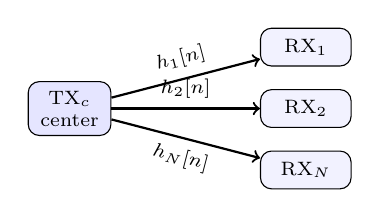
\begin{tikzpicture}[
      tx/.style={draw,rounded corners,fill=Blue!10,minimum width=1.05cm,
                 minimum height=0.55cm,align=center},
      rx/.style={draw,rounded corners,fill=Blue!5,minimum width=1.15cm,
                 minimum height=0.48cm,align=center},
      every node/.style={font=\scriptsize}
    ]
      \node[tx] (tx) at (0,0) {$\mathrm{TX}_{c}$\\center};
      \node[rx] (rx1) at (3.0,0.78) {$\mathrm{RX}_{1}$};
      \node[rx] (rx2) at (3.0,0.00) {$\mathrm{RX}_{2}$};
      \node[rx] (rxn) at (3.0,-0.78) {$\mathrm{RX}_{N}$};
      \draw[->,thick] (tx)--node[above,sloped] {$h_1[n]$} (rx1);
      \draw[->,thick] (tx)--node[above] {$h_2[n]$} (rx2);
      \draw[->,thick] (tx)--node[below,sloped] {$h_N[n]$} (rxn);
    \end{tikzpicture}

    \vspace{0.10cm}
    Fix one center transmitter and collect
    $h_i[n]=H_{i,c}[n]$ for every RX branch $i$.
    The center branches are $\mathrm{TX}_2$, $\mathrm{TX}_3$, and
    $\mathrm{TX}_5$ for $N=3,5,9$ (zero-based $c=1,2,4$).
  \end{block}

  \column{0.54\textwidth}
  \begin{block}{Pairwise RX correlation and decorrelation}
    For each RX pair $(i,j)$, the complex center-TX responses are compared using
    \begin{align*}
      \rho_{ij}&=
      \frac{\sum_n h_i[n]h_j^*[n]}
      {\sqrt{\left(\sum_n|h_i[n]|^2\right)
                   \left(\sum_n|h_j[n]|^2\right)}} ,\\[-0.15em]
      D_{ij}&=1-|\rho_{ij}|.
    \end{align*}
    \textbf{$D_{ij}\approx0$:} similar/correlated RX responses.\par\smallskip
    \textbf{$D_{ij}\approx1$:} distinct/decorrelated RX responses.\par\smallskip
    All RX pairs are summarized using global pooling or a typical local-block
    median.
  \end{block}
\end{columns}

\vspace{0.10cm}
\begin{beamercolorbox}[rounded=true,sep=0.8ex,wd=\linewidth]{takeaway}
  \textbf{Why the center TX?} A fixed source isolates differentiation among RX
  angle/pattern responses. This single-TX metric is not the singular-value
  structure of the full constructed $N\!\times\!N$ MIMO channel.
\end{beamercolorbox}
\end{frame}


\begin{frame}{Worked Example: Center-TX Decorrelation}
\scriptsize
\begin{columns}[T,onlytextwidth]
  \column{0.37\textwidth}
  \begin{block}{Example $3\!\times\!3$ channel}
    Select the center element, $\mathrm{TX}_2$, and observe two channel samples
    from this TX to each RX:
    \[
      \begin{array}{c|c}
        \text{RX branch} & \mathbf h_i=[h_i[1],h_i[2]]\\ \hline
        \mathrm{RX}_1 & [1,\,j]\\
        \mathrm{RX}_2 & [2,\,2j]\\
        \mathrm{RX}_3 & [1,\,-j]
      \end{array}
    \]
    Here, $\mathbf h_2=2\mathbf h_1$: its magnitude is larger, but its
    normalized response has the same shape and phase progression.
  \end{block}

  \column{0.60\textwidth}
  \begin{block}{RX$_1$--RX$_2$: fully correlated}
    \begin{align*}
      \rho_{12}
      &=\frac{1(2)^*+j(2j)^*}
      {\sqrt{(1+1)(4+4)}}
      =\frac{2+2}{4}=1,\\[-0.2em]
      D_{12}&=1-|\rho_{12}|=0.
    \end{align*}
  \end{block}

  \begin{block}{RX$_1$--RX$_3$: fully decorrelated}
    \begin{align*}
      \rho_{13}
      &=\frac{1(1)^*+j(-j)^*}
      {\sqrt{(1+1)(1+1)}}
      =\frac{1-1}{2}=0,\\[-0.2em]
      D_{13}&=1-|\rho_{13}|=1.
    \end{align*}
  \end{block}
\end{columns}

\vspace{-0.07cm}
\begin{beamercolorbox}[rounded=true,sep=0.6ex,wd=\linewidth]{takeaway}
  \centering
  $D_{12}=0$, $D_{13}=1$, and similarly $D_{23}=1$.
  \textbf{The metric measures normalized channel similarity; amplitude scaling
  alone does not create decorrelation.}
\end{beamercolorbox}
\end{frame}



% -----------------------------------------------------------------------------
% Evaluation-equation reference slides
% -----------------------------------------------------------------------------

\begin{frame}[t]{Evaluation Equations I: Channel Construction}
  \footnotesize
  \begin{columns}[T,onlytextwidth]
    \begin{column}{0.49\textwidth}
      \begin{block}{Canonical frequency-domain channel}
        \begin{equation*}
          \mathbf H(f)=\bigl[H_{ij}(f)\bigr]
          \in\mathbb C^{N_R\times N_T}
        \end{equation*}
        \vspace{-1.5ex}
        \begin{equation*}
          \mathbf y(f)=\mathbf H(f)\mathbf x(f)+\mathbf n(f)
        \end{equation*}
      \end{block}

      \begin{block}{Sionna-RT channel coefficient}
        \begin{equation*}
          H_{ij}(f)=\sum_{\ell=1}^{L_{ij}}
          \alpha_{ij,\ell}e^{-j2\pi f\tau_{ij,\ell}}
        \end{equation*}
        \scriptsize $\alpha_{ij,\ell}$ and $\tau_{ij,\ell}$ are the complex
        gain and delay of path $\ell$.
      \end{block}
    \end{column}

    \begin{column}{0.49\textwidth}
      \begin{block}{Singular-value decomposition}
        \begin{equation*}
          \mathbf H=\mathbf U\boldsymbol\Sigma\mathbf V^{H},\qquad
          \boldsymbol\Sigma=\operatorname{diag}(\sigma_1,\ldots,\sigma_q)
        \end{equation*}
        \vspace{-1ex}
        \begin{equation*}
          \sigma_1\geq\cdots\geq\sigma_q\geq0,\qquad
          q=\min(N_R,N_T)
        \end{equation*}
      \end{block}

      \begin{block}{Power-independent channel structure}
        \begin{equation*}
          \widetilde{\mathbf H}
          =\frac{\mathbf H}{\lVert\mathbf H\rVert_{\mathrm F}},\qquad
          \lVert\mathbf H\rVert_{\mathrm F}^{2}
          =\sum_{i,j}|H_{ij}|^2
        \end{equation*}
      \end{block}
    \end{column}
  \end{columns}

  \MethodNote{Raw $\mathbf H$ retains absolute link gain; $\widetilde{\mathbf H}$
  isolates the relative distribution of power among spatial modes.}
\end{frame}


\begin{frame}[t]{Evaluation Equations II: Link Budget and Outage}
  \footnotesize
  \begin{columns}[T,onlytextwidth]
    \begin{column}{0.57\textwidth}
      \begin{block}{Non-coherent combination of simultaneous TX branches}
        \begin{align*}
          P_{\mathrm{RX}}(f)
            &=P_{\mathrm{TX}}\sum_{i=1}^{N_T}|H_i(f)|^2,\\
          P_{\mathrm N}
            &=kTB\,10^{\mathrm{NF}/10},\\
          \gamma(f)
            &=\frac{P_{\mathrm{RX}}(f)}{P_{\mathrm N}}.
        \end{align*}
      \end{block}
    \end{column}

    \begin{column}{0.41\textwidth}
      \begin{block}{Equivalent-SISO link capacity}
        \begin{equation*}
          C_{\mathrm{link}}
          =\frac{1}{N_f}\sum_{m=1}^{N_f}
          \log_2\!\left(1+\gamma(f_m)\right)
        \end{equation*}
        \centering\scriptsize bit/s/Hz
      \end{block}

      \begin{block}{Empirical outage probability}
        \begin{equation*}
          P_{\mathrm{out}}(C_{\mathrm{th}})
          =\frac{1}{N_{\mathrm{obs}}}
          \sum_{u=1}^{N_{\mathrm{obs}}}
          \mathbf 1\!\left\{C_u<C_{\mathrm{th}}\right\}
        \end{equation*}
      \end{block}
    \end{column}
  \end{columns}

  \begin{beamercolorbox}[rounded=true,sep=0.4ex,wd=\linewidth]{caution}
    \scriptsize\textbf{Caution:} $C_{\mathrm{link}}$ retains absolute gain;
    fixed-SNR $C_{\mathrm{MIMO}}$ measures channel structure. The
    1~bit/s/Hz threshold yielded 0\% outage.
  \end{beamercolorbox}
\end{frame}


\begin{frame}[t]{Evaluation Equations III: Conditioning and Effective Rank}
  \footnotesize
  \begin{columns}[T,onlytextwidth]
    \begin{column}{0.48\textwidth}
      \begin{block}{Condition number}
        \begin{equation*}
          \kappa=\frac{\sigma_1}{\sigma_q},\qquad
          \kappa_{\mathrm{dB}}=20\log_{10}\kappa
        \end{equation*}
      \end{block}

      \begin{center}
        \begin{tabular}{c@{\quad$\Longrightarrow$\quad}l}
          $\kappa\rightarrow1$ & balanced modes\\[0.5ex]
          $\kappa\gg1$ & ill-conditioned channel
        \end{tabular}
      \end{center}
    \end{column}

    \begin{column}{0.50\textwidth}
      \begin{block}{Singular-value power fractions}
        \begin{equation*}
          p_i=\frac{\sigma_i^2}{\sum_{k=1}^{q}\sigma_k^2},
          \qquad \sum_{i=1}^{q}p_i=1
        \end{equation*}
      \end{block}

      \begin{block}{Entropy-based effective rank}
        \begin{equation*}
          r_{\mathrm{eff}}
          =\operatorname{exp}\!\left(-\sum_{i=1}^{q}p_i\ln p_i\right),
          \qquad 1\leq r_{\mathrm{eff}}\leq q
        \end{equation*}
      \end{block}
    \end{column}
  \end{columns}

  \Takeaway{Favorable multiplexing has a smaller $\kappa$ and a larger
  $r_{\mathrm{eff}}$. Both depend on singular-value ratios and are unchanged by
  Frobenius normalization.}
\end{frame}


\begin{frame}[t]{Evaluation Equations IV: Spatial Correlation and Decorrelation}
  \scriptsize
  \begin{columns}[T,onlytextwidth]
    \begin{column}{0.50\textwidth}
      \begin{block}{Full-matrix normalized correlation}
        \begin{align*}
          \mathbf R_{\mathrm{RX}}
          &=\mathbf D_{\mathrm{RX}}^{-1/2}
            \mathbf H\mathbf H^H
            \mathbf D_{\mathrm{RX}}^{-1/2},\\
          \mathbf R_{\mathrm{TX}}
          &=\mathbf D_{\mathrm{TX}}^{-1/2}
            \mathbf H^H\mathbf H
            \mathbf D_{\mathrm{TX}}^{-1/2},
        \end{align*}
        where
        \begin{equation*}
          \mathbf D_{\mathrm{RX}}=\operatorname{diag}(\mathbf H\mathbf H^H),
          \quad
          \mathbf D_{\mathrm{TX}}=\operatorname{diag}(\mathbf H^H\mathbf H).
        \end{equation*}
      \end{block}

      Off-diagonal magnitudes quantify response similarity; smaller values
      indicate greater spatial independence.
    \end{column}

    \begin{column}{0.48\textwidth}
      \begin{block}{Pairwise CFR correlation}
        \begin{equation*}
          \rho_{ij}=\frac{\sum_n h_i[n]h_j^*[n]}
          {\sqrt{\left(\sum_n|h_i[n]|^2\right)
          \left(\sum_n|h_j[n]|^2\right)}}
        \end{equation*}
        \vspace{-1.5ex}
        \begin{equation*}
          D_{ij}=1-|\rho_{ij}|,\qquad 0\leq D_{ij}\leq1
        \end{equation*}
      \end{block}

      \begin{block}{Typical-block and amplitude-sensitive summaries}
        \begin{align*}
          D_{ij}^{\mathrm{med}}
            &=1-\operatorname{median}_{w,t}|\rho_{ij}^{(w,t)}|,\\
          Q_{ij}^{\mathrm{raw}}
            &=\frac{1}{N_s}\sum_n|h_i[n]-h_j[n]|^2.
        \end{align*}
      \end{block}
    \end{column}
  \end{columns}

\end{frame}


\begin{frame}[t]{Evaluation Equations V: MIMO Capacity and Scaling}
  \footnotesize
  \begin{columns}[T,onlytextwidth]
    \begin{column}{0.59\textwidth}
      \begin{block}{Equal-power MIMO capacity}
        \begin{align*}
          C_{\mathrm{MIMO}}(\gamma)
          &=\mathbb E_f\!\left[
            \log_2\det\!\left(
              \mathbf I_{N_R}+\frac{\gamma}{N_T}
              \mathbf H\mathbf H^H
            \right)\right]\\
          &=\mathbb E_f\!\left[
            \sum_{i=1}^{q}\log_2\!\left(
              1+\frac{\gamma}{N_T}\sigma_i^2(f)
            \right)\right].
        \end{align*}
      \end{block}
    \end{column}

    \begin{column}{0.39\textwidth}
      \begin{block}{Per-dimension efficiency}
        \begin{equation*}
          \eta_r(N)=\frac{r_{\mathrm{eff}}}{N},
          \qquad
          \eta_C(N)=\frac{C_{\mathrm{MIMO}}}{N}
        \end{equation*}
      \end{block}

      \begin{block}{Operating points in this thesis}
        \scriptsize
        Chapter 2 solver comparison: 20~dB.\\[0.5ex]
        Chapter 3 constructed channels: fixed normalized 10~dB.\\[0.5ex]
        Order study: $N=3,5,9$.
      \end{block}
    \end{column}
  \end{columns}

  \Takeaway{Absolute capacity measures total supported rate; $\eta_r$ and
  $\eta_C$ measure per-dimension use. These are ideal Shannon bounds, not coded
  throughput.}
\end{frame}


\end{document}
